 %+ !TeX encoding = UTF-8
% !TeX spellcheck = fr-FR
%Pourquoi c'est gros ?
\documentclass[a4paper,french,final]{memoir}
\usepackage{shellesc}
\usepackage{babel}
\usepackage[autostyle=true,maxlevel=3]{csquotes}
\usepackage{fontspec}
\usepackage{geometry}
\usepackage[math-style=french,warnings-off={mathtools-colon,mathtools-overbracket}]{unicode-math}
\usepackage{mathtools}
\defaultfontfeatures{Ligatures={TeX},Scale={MatchLowercase}}
\usepackage[amsmath,thmmarks,hyperref]{ntheorem}
\usepackage{cancel}
\usepackage{pifont}
\usepackage{siunitx}
\usepackage[most]{tcolorbox}
\let\ordinal\relax
\usepackage{fmtcount}
\usepackage{enumitem}
\usepackage{booktabs}
\usepackage{nicematrix}
\usepackage{ragged2e}  % Permet la césure dans les marges
\usepackage{tikz}
\usetikzlibrary{calc,trees,positioning,arrows,fit,shapes,calc}
\usepackage[justification=centering]{subcaption}
\usepackage{float}
\usepackage{placeins}
\usepackage{lualatex-math}
\usepackage{graphicx}
\usepackage{svg}
% \usepackage{lua-typo}
%\usepackage[xindy]{imakeidx}
%\makeindex[options= -M index -C utf8 -L french]
%\usepackage[totoc]{idxlayout}
\usepackage{varioref}
\usepackage{nameref}
\usepackage[unicode,naturalnames,plainpages=false,pdfencoding=auto,hidelinks]{hyperref}
\usepackage[noabbrev,nameinlink]{cleveref} % Names references automatically. Load after hyperref.

\hypersetup{pdfprintscaling=None}
\AtBeginDocument{\let\savedemptyset\emptyset} % 
\AtBeginDocument{\let\emptyset\varnothing} % 
\AtBeginDocument{\let\savedphi\phi} % 
\AtBeginDocument{\let\phi\varphi} %
\AtBeginDocument{\let\varphi\savedphi} % 
\AtBeginDocument{\let\savedleq\leq} % 
\AtBeginDocument{\let\savedgeq\geq} %
\AtBeginDocument{\let\leq\leqslant} % 
\AtBeginDocument{\let\geq\geqslant} %
\newcommand{\paral}{\mathrel{\!/\mkern-5mu/\!}} % \parallel existe déjà : || vs //
\makeatletter
\renewcommand*{\thepart}{\@arabic\c@part}
\renewcommand*{\thechapter}{\@Roman\c@chapter}
\NewCommandCopy{\oldthechapter}{\thechapter}
\newcommand*{\theauthor}{\@author}
\newcommand*{\thetitle}{\@title}
\newcommand*{\thedate}{\@date}
\renewcommand*{\cftchapterpresnum}{\@chapapp~}
\renewcommand{\xmapsto}[2][]{\mathrel{\mathpalette\xmapsto@{{#1}{#2}}}}
\renewcommand{\xmapsto}[2][]{\mathrel{\mathpalette\xmapsto@{{#1}{#2}}}}
\newcommand{\xmapsto@}[2]{\xmapsto@@{#1}#2}
\newcommand{\xmapsto@@}[3]{%
  \begingroup
  \sbox\z@{$\m@th#1\mathop{}\limits_{\;#2\;}^{\;#3\;}$}%
  \mathop{\Uhextensible width \wd\z@ 0 "27FC}_{#2}^{#3}%
  \endgroup
}
\renewcommand{\xLeftrightarrow}[2][]{\mathrel{\mathpalette\xLeftrightarrow@{{#1}{#2}}}}
\newcommand{\xLeftrightarrow@}[2]{\xLeftrightarrow@@{#1}#2}
\newcommand{\xLeftrightarrow@@}[3]{%
  \begingroup
  \sbox\z@{$\m@th#1\mathop{}\limits_{\;#2\;}^{\;#3\;}$}%
  \mathop{\Uhextensible width \wd\z@ 0 "027FA}_{#2}^{#3}% 027FA code for long left right double arrow in unicode-math-table.tex 
  \endgroup
}
\renewcommand{\xrightarrow}[2][]{\mathrel{\mathpalette\xrightarrow@{{#1}{#2}}}}
\newcommand{\xrightarrow@}[2]{\xrightarrow@@{#1}#2}
\newcommand{\xrightarrow@@}[3]{%
  \begingroup
  \sbox\z@{$\m@th#1\mathop{}\limits_{\;#2\;}^{\;#3\;}$}%
  \mathop{\Uhextensible width \wd\z@ 0 "027F6}_{#2}^{#3}% 027F6 code for long left right  arrow in unicode-math-table.tex
  \endgroup
}
\AtBeginDocument{%
  \check@mathfonts
  \iffontchar\textfont\tw@\string"23AF
    \renewcommand{\relbar}{\mathrel\harrowextender}%
  \else
    \Umathcharnumdef\std@minus\Umathcodenum`-
  \fi}
\newcounter{proofpart}
\newcommand{\proofpart}{\@ifstar{\@proofpart}{\@@proofpart}}

\newcommand{\@proofpart}[1]{%
  \if\detokenize{#1}\relax\else{
  \par
  \addvspace{\medskipamount}%
  \noindent \itshape%
  {#1~:\par\nobreak\smallskip}%
  \normalfont
  \@afterheading
}\fi
}

\newcommand{\@@proofpart}[1]{%
  \par
  \addvspace{\medskipamount}%
  \stepcounter{proofpart}%
  \noindent Partie \theproofpart~:~\itshape%
  \if\detokenize{#1}\relax%
  \else{#1.}\fi%
  \par\nobreak\smallskip
  \normalfont
  \@afterheading
}
\AtBeginDocument{% placeins code for [section] adapted for subsection.
  \expandafter\renewcommand\expandafter\subsection\expandafter
    {\expandafter\@fb@secFB\subsection}%
  \newcommand\@fb@secFB{\FloatBarrier
    \gdef\@fb@afterHHook{\@fb@topbarrier \gdef\@fb@afterHHook{}}}%
  \g@addto@macro\@afterheading{\@fb@afterHHook}%
  \gdef\@fb@afterHHook{}%
}
\makeatother
\newcommand{\scroman}[1]{\addfontfeature{SmallCapsFeatures={LetterSpace=0}}\textsc{\roman{#1}}}
% 2 lignes pour localiser les overfull hbox et vbox dans le log
\showboxdepth=\maxdimen
\showboxbreadth=\maxdimen
\newcounter{PageNumberBeforeMainmatter}
\let\LaTeXStandardMainmatter\mainmatter%
\renewcommand{\mainmatter}{%
\setcounter{PageNumberBeforeMainmatter}{\number\value{page}}%
\LaTeXStandardMainmatter%
}%
\let\LaTeXStandardFrontmatter\frontmatter
\renewcommand{\frontmatter}{%
  \LaTeXStandardFrontmatter%
  \renewcommand*{\thepage}{\texorpdfstring{\scroman{page}}{\roman{page}}}%
  }
\let\LaTeXStandardAppendixPage\appendixpage
\renewcommand{\appendixpage}{
\openany
\renewcommand*{\cftchapterpresnum}{Annexe~}
\LaTeXStandardAppendixPage%
\setcounter{page}{\number\value{PageNumberBeforeMainmatter}+1}
    \renewcommand*{\thepage}{\texorpdfstring{\scroman{page}}{\roman{page}}}
  	\addtocontents{toc}{\protect\renewcommand\protect\cftchapterpresnum{\appendixname~}}
  }%%

%\usepackage[backend=biber,style=alphabetic]{biblatex}
\renewbibmacro*{date}{%
	\printdate
	\iffieldundef{origyear}{%
	}{%
		\setunit*{\addspace}%
		\printtext[parens]{\printorigdate}%
	}%
}
\addbibresource{references.bib}
\renewcommand*{\Rnfont}{\scshape}
\DefineBibliographyStrings{french}{urlseen={consult\'e~le}}
%%% Local Variables:
%%% mode: latex
%%% TeX-master: "../main"
%%% End:

%%%%%%%%%%%%%%%%%%%%%%%%%%%%%
%   PAGE DE GARDE            %
%%%%%%%%%%%%%%%%%%%%%%%%%%%%%
%%
\newcommand{\HRule}{\rule{\linewidth}{0.5mm}} % trait, régler épaisseur
\newcommand*{\theuniversity}{Université de Toulon}
\newcommand*{\theyearname}{Master d'informatique, développement et ingéniérie des données (\bsc{did}),
1\textsuperscript{re}~année}
%\newcommand*{\thesupervisor}{Prénom \bsc{Nom}}
\author{Jason~\bsc{Laffaille},~Théo~\bsc{Hafsaoui}~\&~Tom~\bsc{Domenge}}
\title{Rapport de projet collaboratif \\
Création d'un logiciel de gestion d'emploi du temps}
%%
%%%%%%%%%%%%%%%%%%%%%%%%%%%%%%%%%%%%%%%%%%%%%%
%   	Marges et note en marge.   			 %
%%%%%%%%%%%%%%%%%%%%%%%%%%%%%%%%%%%%%%%%%%%%%%
%%
\setheaderspaces{*}{*}{*}
\setlrmargins{*}{*}{*}
\setheadfoot{\headheight}{\footskip}
\checkandfixthelayout[nearest]
\renewcommand*{\sideparfont}{\itshape\footnotesize}
\renewcommand*{\sideparform}{\ifmemtortm\RaggedRight\else\RaggedLeft\fi%
  \mathsurround=1pt%
  \parindent=0pt%
}
\epigraphfontsize{\footnotesize}
%%
%%%%%%%%%%%%%%%%%%%%%%%%%%%%%%%%%%%%%%%%%%%%%%%%
%            Numérotation (classe memoir)       %
%%%%%%%%%%%%%%%%%%%%%%%%%%%%%%%%%%%%%%%%%%%%%%%%
%%
\setsecnumdepth{subsubsection}
\renewcommand{\cftpartaftersnum}{.}
\renewcommand{\cftchapteraftersnum}{.}
\renewcommand{\cftpartdotsep}{\cftdotsep}
% \renewcommand{\cftchapterdotsep}{\cftdotsep}% Chapters should use dots in ToC
\renewcommand\cftpartpresnum{Partie~}
\addtolength{\cftpartnumwidth}{3em}
\addtolength{\cftchapternumwidth}{6.5em}
\aliaspagestyle{title}{empty}
\aliaspagestyle{part}{empty}
\addto\captionsfrench{\renewcommand{\appendixpagename}{Annexes}}
\addto\captionsfrench{\renewcommand{\appendixtocname}{Annexes}}
\renewcommand\partnamefont{\normalfont\huge\scshape}
%\renewcommand\partnumfont{\Large\scshape}
%%
%%%%%%%%%%%%%%%%%%%%%%%%%%%%%%%%%%%%%%%%%%%%%%%%
%            Polices                           %
%%%%%%%%%%%%%%%%%%%%%%%%%%%%%%%%%%%%%%%%%%%%%%%%
%%
\lefthyphenmin=3
\righthyphenmin=3
\newfontfeature{Microtype}{protrusion=default;}%
\directlua{fonts.protrusions.setups.default.stretch=1.5}
\setmainfont[Microtype,Ligatures={Common, Discretionary,TeX},ItalicFeatures={ScaleAgain=1.142847558},SmallCapsFeatures={LetterSpace=7,
    Renderer = Basic,
    Letters = SmallCaps}]{TeX Gyre Pagella}

\setmonofont{inconsolata}
\setmathfont{Asana Math}
\setmathfont[range={"0000-"0001,"0020-"007E,
                    "00A0,"00A7-"00A8,"00AC,"00AF,"00B1,"00B4-"00B5,"00B7,
                    "00D7,"00F7,
                    "0131,
                    "0237,"02C6-"02C7,"02D8-"02DA,"02DC,
                    "0300-"030C,"030F,"0311,"0323-"0325,"032E-"0332,"0338,
                    "0391-"0393,"0395-"03A1,"03A3-"03A8,"03B1-"03BB,
                    "03BD-"03C1,"03C3-"03C9,"03D1,"03D5-"03D6,"03F5,
                    "2016,"2018-"2019,"2021,"2026-"202C,"2032-"2037,"2044,
                    "2057,"20D6-"20D7,"20DB-"20DD,"20E1,"20EE-"20EF,
                    "210B-"210C,"210E-"2113,"2118,"211B-"211C,"2126-"2128,
                    "212C-"212D,"2130-"2131,"2133,"2135,"2190-"2199,
                    "21A4,"21A6,"21A9-"21AA,"21BC-"21CC,"21D0-"21D5,
                    "2200,"2202-"2209,"220B-"220C,"220F-"2213,"2215-"221E,
                    "2223,"2225,"2227-"222E,"2234-"2235,"2237-"223D,
                    "2240-"224C,"2260-"2269,"226E-"2279,"2282-"228B,"228E,
                    "2291-"2292,"2295-"2299,"22A2-"22A5,"22C0-"22C5,
                    "22DC-"22DD,"22EF,"22F0-"22F1,
                    "2308-"230B,"2320-"2321,"2329-"232A,"239B-"23AE,
                    "23DC-"23DF,
                    "27E8-"27E9,"27F5-"27FE,"2A0C,"2B1A,
                    "1D400-"1D433,"1D49C,"1D49E-"1D49F,"1D4A2,"1D4A5-"1D4A6,
                    "1D4A9-"1D4AC,"1D4AE-"1D4B5,"1D4D0-"1D4E9,"1D504-"1D505,
                    "1D507-"1D50A,"1D50D-"1D514,"1D516-"1D51C,"1D51E-"1D537,
                    "1D56C-"1D59F,"1D6A8-"1D6B8,"1D6BA-"1D6D2,"1D6D4-"1D6DD,
                    "1D6DF,"1D6E1,"1D7CE-"1D7D7},Path={backend_code/}]{euler.otf}
\setmathfont[range={bfup/{latin, Latin, greek, Greek,num}, frak, bffrak,up/num},
             script-features={}, sscript-features={},Path={backend_code/}]{euler.otf}
\setmathfont[range={it, bfit,
                    sfup, sfit, bfsfup, bfsfit, tt,}
                  ]{Asana Math}
\setmathfont[range={bb},Scale=MatchUppercase]{STIX Two Math}
\setmathfont[range={scr,"2980-"29FF,"27C0-"27E7,"27E9-"27FF,"222E-"2233,\sum,\int,\prod},Scale=MatchUppercase]{TeX Gyre Pagella Math}
\setmathfont[range={cal,bfcal,\setminus}, Scale=MatchUppercase, Alternate]{Asana Math}
\everydisplay{\Umathoperatorsize\displaystyle=5ex}
\usepackage[verbose=silent,final]{microtype}
\protrudechars=2
\adjustspacing=2
%%
%%%%%%%%%%%%%%%%%%%%%%%%%%%%%%%%%%%%%%%%%%%%%%%%
%            Utilitaires                       %
%%%%%%%%%%%%%%%%%%%%%%%%%%%%%%%%%%%%%%%%%%%%%%%%
%%
\newcommand{\siecle}[1]{\addfontfeature{SmallCapsFeatures={LetterSpace=0}}\textsc{\romannumeral#1}%
\ifnum#1=1%
\up{e}%
\else%
\up{er}\fi%
\addfontfeature{SmallCapsFeatures={LetterSpace=7}}%
}

\graphicspath{{./figures/}}
%\tikzset{|/.tip={Bar[width=.8ex,round]}}
%\usetikzlibrary{arrows.meta}

\begin{document}
\begin{titlingpage}
\hypersetup{pageanchor=false}
\vspace*{\fill}%
\begin{center}
  \vspace*{\fill}%
\makebox[\linewidth]{\HRule} % demande à latex l'espace pour le trait
\parbox[t]{\linewidth}{\addvspace{\parskip} % on ajoute ce qu'il faut d'espace pour sous le trait
\centering\huge\bfseries\thetitle}
 \null%Espace obligatoire pour LaTeX (boite vide) sinon l'espace est ignoré
\vspace*{\parskip}
\makebox[\linewidth]{\HRule}
\vspace*{\fill}
\par LOGOS
\vspace{\fill}
\par \Large Rédigé par \theauthor\par% Supervisé par \thesupervisor \par
\vspace*{\fill}
\large{\theyearname.\par \theuniversity, Version du \thedate.}
\end{center}

\end{titlingpage}
\frontmatter
\tableofcontents
\chapter{Introduction}
\section{Avant-propos}
\begin{quote}
    Ce rapport est le résultat du travail réalisé sur le projet du premier semestre du M1 master info d'ingénierie
logicielle. ce projet consiste en la réalisation sur 11 semaines d'un logiciel d'emploi du temps avec un fort
accent sur la gestion de projet agile avec le soutien de professionnels (techlead/buisness analyst) de Sopra.
Plus particulièrement, un effort important a été réalisé afin d'utiliser des méthodes de gestion
moderne avec, github, pull request, kanban, intégration continue, le tout en parfaite synchronisation avec les
possibilité offerte par Github.


Pour résumer, ce projet consiste en la réalisation d'une application similaire à hyperPlanning avec une gestion
de base de donne et d'utilisateur sur java avec le SGBD de notre choix.
\end{quote}

\section{Rencontre des acteurs}
Dans le cadre de l'appropriation du sujet, nous avons décidé, dès que possible, d'interroger les acteurs primaires
d'\texttt{Hyperplanning} dans notre université et à l'étranger. Pour ce faire, nous avons utilisé plusieurs mediums, D'abord bien sur des discussions physiques, nous remercions d'ailleurs M.\texttt{VIA} qui a pris le temps de nous parler deux fois, ensuite avec des formulaires en ligne. Ces retours furent riches d'information ; les utilisateurs d'\texttt{Hyperplanning}  avait une tendance naturelle à se concentrer sur leur frustration et peu sur les composantes essentielle et utile pour eux, un travail de synthèse fut donc nécessaire pour la création des UC (cf.\ref{fig:diaguc}).
\begin{center}
        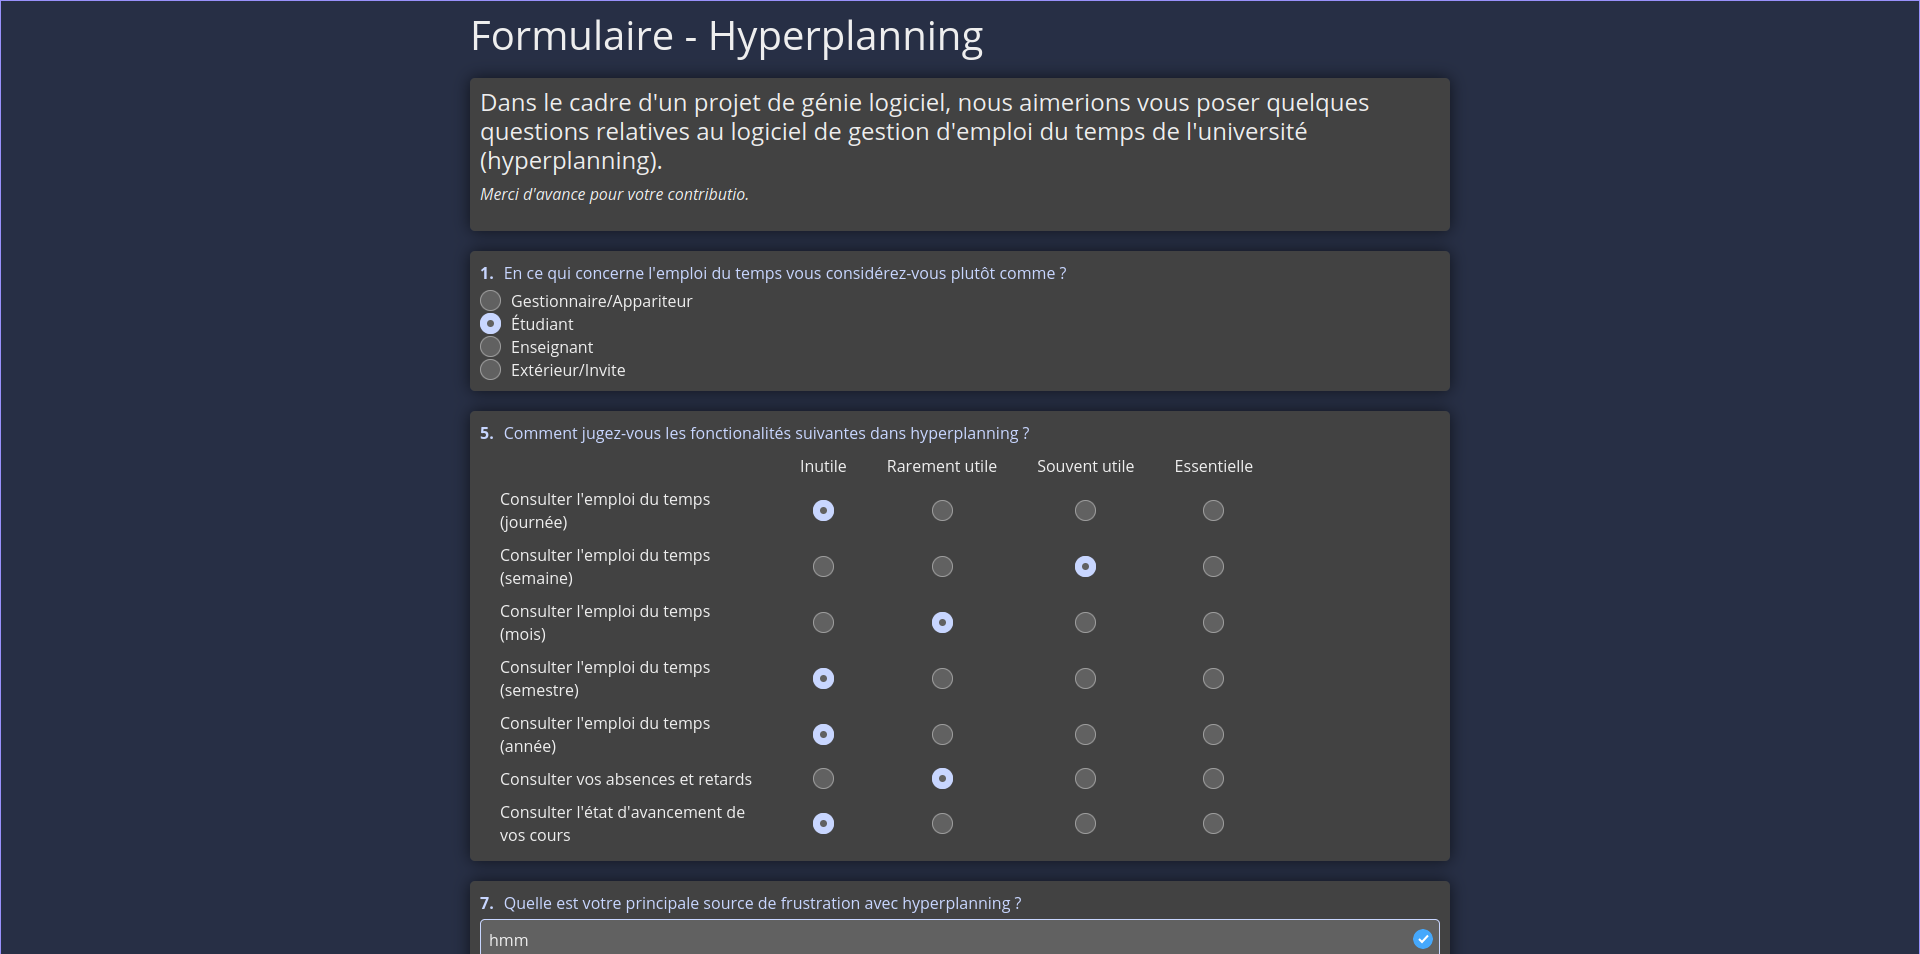
\includegraphics[width=0.8\textwidth]{figures/Form.png}
\end{center}


Ci-dessous les retours synthétisés des différents acteurs principaux.

\subsection{Enseignants}
D'après les retours et les avis différents reçu par les Acteurs Enseignants d'\texttt{Hyperplanning}, on peut en extraire de multiples composantes essentielles quant à l'utilisation du logiciel,
tel que la consultation d'emplois du temps (par jour / semaine / mois), en revanche l'avis de consulter son emploi du temps au semestre ou à l'année était en faveur de l'indifférence, il en est de même pour consulter la progression d'un cours, ainsi que communiquer avec les étudiants directement depuis \texttt{Hyperplanning}.
Contre toutes attentes, la réservation d'une salle est également sujet d'indifférence, puisque chaque enseignant doit d'abord notifier le Gestionnaire de la promotion pour y communiquer les changements au Gestionnaire du Planning. Pour conclure, nous avons demandé aux Acteurs, quelles sont vos principales frustrations quant à l'utilisation d'\texttt{Hyperplanning}, leur réponse été davantage tourné côté gestion qui traîne parfois à les notifier. Une idée a aussi été évoquée d'initier un système de notification automatique pour les étudiants et les enseignants en cas de changement soudain ou report de cours.
On nous a aussi informés que si un Enseignant Chercheur souhaitait réserver une salle pour une réunion, hors du cadre d'une quelconque formation, elle ne pouvait être renseignée sur \texttt{Hyperplanning} sans créer une autre cohorte hors de la formation, donc pourquoi pas intégrer une possibilité de renseigner les réunions de différents intervenants.
Finalement, un dernier point sur la facilité d'utilisation nous a été reporté, tel que le choix de filtrer les différentes informations de l'emploi du temps, filtrer par type d'enseignement (CM, TD, TP), ou simplement le numéro d'un groupe, des filtres qui ne sont actuellement pas possibles avec \texttt{Hyperplanning}.
Les réponses obtenues sont riches en informations sous leur contexte d'utilisation respectif.

\subsection{Étudiant}
Une attention particulière fut apportée sur le profile des étudiants sondés, avec une diversité de statue professionnelle, d'U.F.R, mais aussi géographique avec des étudiants étrangers.
Les résultats sont similaires à ceux des étudiants avec une nette préférence pour l'affichage de l'emploi du temps de la journée et de la semaine. le reste des fonctionnalités est jugée  "\emph{inutile}" ce qui peut sembler intuitive concernant un emploi du temps, a noté que beaucoup de fonctionnalité sont inconnues des étudiants, comme l'e.d.t des salles ou l'accès a e.d.t d'autre promotion.
\subsection{Gestionnaire}
Le gestionnaire, lui, nous a fait part de son souhait d'une interface plus sobre, tout en conservant la possibilité de visualiser en direct les emplois du temps de tous les groupes. Il nous a indiqué que la gestion des disponibilités des enseignants était un processus transverse, de sorte que nous n'avons pas retenu cette fonctionnalité dans notre logiciel. 
\mainmatter
\chapter{Exigences}\label{chap:exigence}
\section{Utilisateur
}
\begin{quote}
    Un utilisateur doit pouvoir voir son emploi du temps
\end{quote}
\line(1,0){450}

\begin{quote}
    Un utilisateur doit pouvoir se connecter de manière sécuriser à son emploi du temps
\end{quote}
\line(1,0){450}

\begin{quote}
    Un utilisateur doit pouvoir voir l'emploi du temps de la semaine prochaine
\end{quote}
\line(1,0){450}

\begin{quote}
    Un utilisateur doit pouvoir voir l'emploi du temps de la semaine précédente
\end{quote}
\line(1,0){450}

\begin{quote}
    Un utilisateur doit pouvoir voir l'avancement d'un cours.
\end{quote}
\line(1,0){450}


\section{Administrateur}
\begin{quote}
    L'administrateur doit pouvoir se connecter de manière sécuriser à son emploi du temps
\end{quote}
\line(1,0){450}

\begin{quote}
    L'administrateur doit pouvoir voir l'emploi du temps d'un utilisateur.
\end{quote}
\line(1,0){450}

\begin{quote}
    L'administrateur doit pouvoir voir l'emploi du temps d'une salle.
\end{quote}
\line(1,0){450}

\begin{quote}
    L'administrateur doit pouvoir voir l'emploi du temps d'un enseignant.
\end{quote}
\line(1,0){450}

\begin{quote}
    L'administrateur doit pouvoir supprimer un créneau
\end{quote}
\line(1,0){450}


\begin{quote}
    L'administrateur doit pouvoir modifier un créneau
\end{quote}
\line(1,0){450}

\begin{quote}
    L'administrateur doit pouvoir ajouter un créneau
\end{quote}
\line(1,0){450}

\begin{quote}
    L'administrateur doit pouvoir lire un créneau
\end{quote}
\line(1,0){450}


\section{Professeur}

\begin{quote}
    Un professeur doit pouvoir voir son emploi du temps
\end{quote}
\line(1,0){450}


\begin{quote}
    Un cours doit pouvoir avoir plusieurs enseignants
\end{quote}
\line(1,0){450}

\begin{quote}
    Un professeur doit pouvoir se connecter de manière sécurisée à son emploi du temps
\end{quote}
\line(1,0){450}

\begin{quote}
    Un professeur doit pouvoir voir l'emploi du temps de la semaine prochaine
\end{quote}
\line(1,0){450}

\begin{quote}
    Un professeur doit pouvoir voir l'emploi du temps de la semaine précédente
\end{quote}
\line(1,0){450}

\begin{quote}
    Un professeur doit pouvoir voir l'avancer d'un de ces cours
\end{quote}
\line(1,0){450}

\begin{quote}
    Un professeur doit pouvoir renseigner une indisponibilité
\end{quote}
\line(1,0){450}


\section{Système}
\begin{quote}
    Le système doit se charger en moins de 3 seconde
\end{quote}
\line(1,0){450}

\begin{quote}
    Le système doit assurer la cohérence de l'emploi du temps avec:
    \begin{enumerate}
        \item Un enseignant ne peut être sur deux créneaux au même instant
        \item Une promotion ne peut être sur deux créneaux au même instant
        \item Assurer l'unicité des matières
        \item Assurer l'unicité des enseignants
        \item Assurer l'unicité des promotions.
    \end{enumerate}
\end{quote}
\line(1,0){450}


\chapter{Axe fonctionnel}



\renewcommand\numberlinebox[2]{#2} % for sections
\renewcommand\chapternumberlinebox[2]{#2} % for chapters 

L'axe fonctionnel se concentre sur les fonctionnalités qu'offrent notre logiciel, plus spécifiquement le but de cette partie est de dégager les \emph{acteurs} du système, les \emph{service} que le système doit rendre aux acteurs et les interactions entre les deux.

\section{Diagramme de contexte statique}
face à cet objectif, nous devons commencer par un diagramme de contexte statique, ce diagramme isole le système et met en lumière les acteurs
qui interagisse avec lui.
\begin{center}
    \includesvg[width=0.7\columnwidth]{figures/statique.svg}
\end{center}

Ce diagramme a été réaliser grâce aux attendus du projet ainsi que les interviews réalisées au début de ce rapport.
Deux choses sont à noter de ce diagramme, premièrement les cardinalités sont absentes, car très probablement identiques.
Deuxièmement, les acteurs secondaires sont aussi absents, en effet il nous apparaît précipité de définir nos choix d'implantations et de subir involontairement une dette technique, dans une étape aussi précoce de la modélisation.

\section{Diagramme de cas d’utilisation}
Maintenant que les acteurs sont définis, il est nécessaire de mettre en évidence les
service rendue par notre système, afin d'éviter encore une fois un choix précoce nous 
allons commencer ce premier Cas d'usage par une approximation de la réalité que nous
raffinerons plus tard.
\begin{figure}
    \centering
    \includesvg[width=0.7\columnwidth]{figures/use_case.svg}
    \caption{Diagramme de cas d'usage}
    \label{fig:my_label}
\end{figure}


Bien sûr, il ne s'agit que d'une approximation, mais deux choses importantes sont à notées:
\begin{enumerate}
    \item L'héritage entre acteurs. ici nous ne parlons pas forcement d'implantation mais
    bien d'un héritage contraint par les fonctionnalités, il s'agit d'un héritage artificielle car bien sur un Enseignant n'est pas \emph{exactement} un Étudiant. Subtilité
    que nous étudierons dans les diagrammes suivant.
    \item Le faible nombres UC. Ce faible nombre est un choix de granularité grossier
    pour mettre en évidence les lien entre acteurs. Même si au final cela représente
    tout nos objectifs pour ce projet.
\end{enumerate}

Bien sur l'étape suivante, est l'écriture des scénario nominaux mais c'est le domaine
de l'axe statique. Néanmoins si nous soulignions l'importance de cette étapes c'est parce que c'est grâce a elle que nous avons trouver les prochaine UC as un niveaux de granularité
qui nous satisfaisait. Aussi si la structure du rapport peut sembler chronologique il n'en n'est rien la conception as était un meli-melo avec chaque étapes qui soulevait des ambiguïté et qui mettait en lumière des erreur faite dans les étapes précédente, ceci sans
inclure l'implantation qui bien sur nous forcis a faire de nombreux changement.
\section{Paquetage}
Cette Partie est celle ou nous obtenons la version final de nos UC. L'objectif ici est diamétralement diffèrent du premier UC, en effet si précédemment nous souhaitions unir est trouver les fonctionnalité en commun, ici nous supposons chaque acteur unique. C'est a dire
que le système a pour unique objectif de le servir lui, cette approche a pour desseins
de faire ressortir les différence, et surtout de s'assurer de la cohérence de notre première
UC avec la réalité des besoins de \emph{chaque} acteurs.

\subsection{Étudiant}

\begin{center}
    \includesvg[width=0.5\columnwidth]{figures/UCstudent.svg}
\end{center}

Cette UC est sans doute la plus connue des membres de l'équipe. En effet étant \emph{Etudiants}
il s'agissait sans doute du plus facile à cerner. Cette UC n'as pas toujours était aussi
simple en effet lors des première itération nous avions une version beaucoup plus précise,
mais inutilement précis, particulièrement en ce que nous avons appeler les \emph{Filtre} qui ne sont au final que diffèrent vue d'un même EDT préciser tout ces diffèrent filtre ne polluer pas seulement la lisibilité du diagramme, elle rendait le développement imminent plus rigide
après tout devions nous vraiment avoir une vison journalière ? La réponse est non, en tout cas c'est le choix de l'équipe après avoir décider d'abandonner ces UC trop complexe.


\begin{center}
    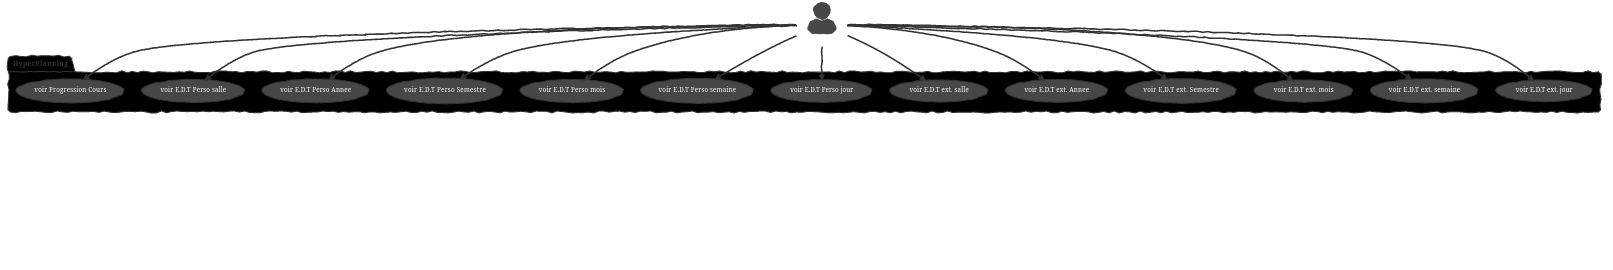
\includegraphics[width=0.9\columnwidth]{figures/OldEtudiant.png}
\end{center}


\subsection{Enseignant}
L'enseignant est au final beaucoup plus similaire a l'étudiant du point vue fonctionnelle que l'on aurais pus se l'imaginer. En effet même si en terme d'implantation
étudiant et professeur sont deux objet très diffèrent, car bien sur un professeur est intrinsèquement lier a la notions de cours est donc d'emploi du temps au contraire
d'un étudiant lui qui n'est lier que par ça promotion.
Cependant malgré cette différence de  nature les deux possède deux UC identique. Une nuance est néanmoins as apporter a cause des interview, puisque les deux n'apporte
pas la même importance au fonctionnalité avec ici une nette augmentation de l'intérêt pour la progression du cours.
\begin{center}
    \includesvg[width=0.5\columnwidth]{figures/UcTeacher.svg}
\end{center}
\subsection{Extérieur}
\begin{center}
    \includesvg[width=0.5\columnwidth]{figures/UCguest.svg}
\end{center}
l'extérieur est aussi un acteur intéressant, tant sont existence n'est pas nécessaire. c'est fonctionnalité elle sont la aussi similaires aux autres utilisateurs
avec évidement la suppression des UC EDT PERSO et les UC de progression de cours qui n'ont aucune raison d'être pour une personne qui n'as a a priori aucun cours.
Je l'ai donc sont existence as etait remis en question, mais il as était garder tant il est au final une étapes afin de réaliser toute les fonctionnalité du Gestionnaire.
\subsection{Gestionnaire}
\begin{center}
    \includesvg[width=0.5\columnwidth]{figures/UCadmin.svg}
\end{center}
Le gestionnaire comme dit précédemment n'est en réalité qu'un hybride entre les utilisateur et les extérieur, avec la possibilité de voir l'emploi du temps d'un étudiant,
d'un enseignant ou d'une promotion, cette diversité de vision est nous l'avons compris au fil de nos discussion un élément crucial dans le travaille de M.\texttt{VIA}.
aussi nous avons compris qu'il était donc nécessaire d'avoir des UC de lecture EDT solide, cependant pendant le developement le choix as était fait d'abandonner la vision
par étudiants et par enseignants, nous croyons en effet que le rôle du gestionnaire n'est pas la gestion des individus mais la gestion de promotion, il s'agit aussi pour
nous d'un raccourcis car cela nous permet d'éviter la création de feature inutile, qui surchargerait inutilement l'interface.

Enfin bien sur l'une des feature essentielle pour le gestionnaire et la modification, suppression, et l'ajout de cours. il s'agit la d'une partie nous le savons
complexe est qui pourrait recevoir une myriad d'option pour simplifier la vie du gestionnaire, cependant cette richesse d'option seras réserver pour la roadmap et
les amélioration potentielle puisque nous pensons d'abord essentielle d'avoir le coeur de la gestion avant leur amélioration potentielle, d'où la simple
UC CRUD qui est nous le savons bien plus complexe que sont court nom pourrait laisser entendre.


\chapter{Axe statique}\label{chap:statique}
\headepigraph{\foreignlanguage{american}{To build a software that your users understand, capture the language of th[ose] users in~a~class~diagram.}}{Michael Jesse Chonoles, \normalfont in~\textit{UML 2 for Dummies}}

L'axe dynamique décrit l'aspect structurel de notre système, les classes qui le composent et leur relation.
Une fois les exigences définies, une grande partie du temps avec les intervenants a consisté à dégager les éléments de la statique de notre système. 
Ainsi, le modèle change selon que l'on restreint un cours à un ou plusieurs enseignants: Toute la modélisation de la base de données en dépend également. Les retours du gestionnaire en la matière se sont montrés 
particulièrement intéressants, et nous ont permis de dégager la hiérarchie de classe finale de notre projet. 

\section{Entités et objets métier}
Comme nous aurons l'occasion de revenir là-dessus, l'une des clés de voûte de notre conception et la phrase ci-dessous. c'est un élément important,
il synthétise toutes les informations nécessaires pour avoir un \emph{Cours}.
\begin{quote}
    Le vendredi 25 novembre 2021 \textit{de neuf heures à midi}, les étudiants du \textit{Master 1 Informatique} assistent à  une séance de \textit{travaux dirigés}, dispensée par \textit{MM. \bsc{Mallofre} et \bsc{Loiseau}} dans le cadre du module \textit{projet collaboratif (I~143)}, en salle \textit{U.001}.
\end{quote}
Les informations en \emph{italique} sont propres à chaque cours, mais l'on peut déjà en dégager des informations comme des contraintes
\begin{enumerate}
    \item  spatio-temporelles: dans une certaine salle, à une heure donnée
    \item  de multiplicité, pour les enseignants
    \item de dépendance à d'autres objets, les noms d'enseignants et de promotions étant vraisemblablement présents sur plusieurs cours
\end{enumerate}
\clearpage
Forts de ce constat, nous et après de multiple modification, nous avons obtenue ce diagramme:
\begin{figure}[!h]
    \centering
    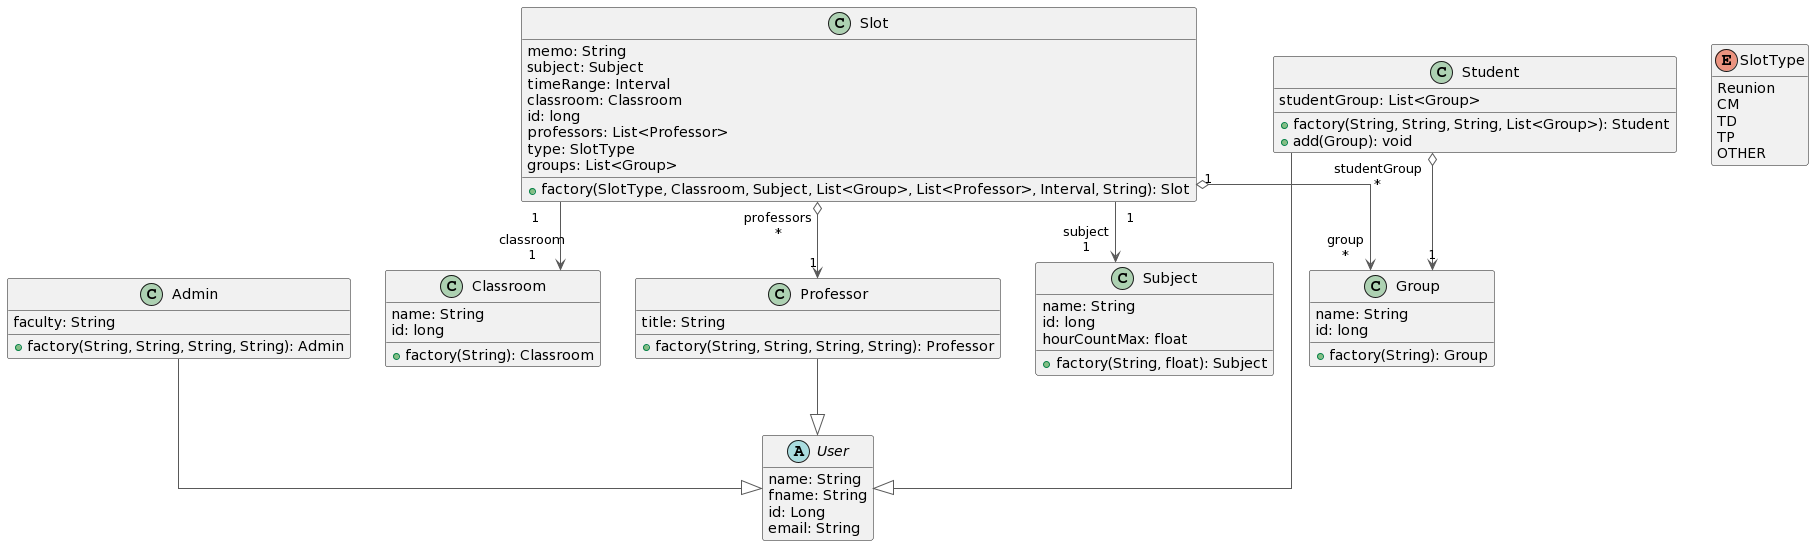
\includegraphics[width=1.1\textwidth]{figures/diag_classe.png}
    \caption{Diagramme de classes des entités}
    \label{fig:diag_classes}
\end{figure}

Bien sûr, il s'agit d'un diagramme plutôt vaste puisqu'il regroupe tout notre système, aussi l'une des étapes réalisées afin de vraiment comprendre
ce diagramme est la scission en \emph{paquets}. Ce paquetage est réalisé d'abord de manière sémantique, on réunit les classes avec des rôles en commun, ensuite 
on essaie de réduire au maximum les relation et cardinalités entre paquets. de ces règles simples, on en obtient la séparation ci-dessous.
\begin{center}
    \includesvg[width=0.9\columnwidth]{figures/packet.svg}
\end{center}

A notée que ce diagramme n'est pas le plus récent, mais ici, il servira de support pour
expliquer certains des changements fait pendant le projet, dans nos choix de conception.


 \begin{enumerate}
    \item \textbf{Usager:}
Le packet Usager regroupe tous les acteurs primaires de notre système, les relations entre classe sont principalement des relations d'héritage.
Ainsi est de manière logique \emph{un Enseignant est un utilisateur}, la seule exeption a ce raisonnement est l'invite d'où sa disparition dans le diagramme final.
À la fin, la seule à interagir en dehors du paquet est \emph{Usager} avec un lien $1\dots N$.


\begin{center}
    \includesvg[width=0.4\columnwidth]{figures/Slot.svg}
\end{center}


    \item \textbf{Cours: }Ce packet regroupe les classes composant un créneau, autrement
    appelé cours ou Slot en anglais. la ou le packet \emph{Usager} était très uniforme dans les
    relation entre ces classes, le paquet \emph{Creneaux} est beaucoup plus hétéroclite. Pour commencer par le plus simple, nous avons les relations entre \emph{Matière} et \emph{Classe} avec
    la classe \emph{Cours}, ces relations sont simples, car il s'agit juste d'un lien $1\dots1$.
    cela s'explique par le bon sens, un cours sans sujet ni lieu n'a aucune raison d'exister et réciproquement. Le lien entre un \emph{Enseignant} et un \emph{Cours} est un peu plus complexe, déjà enseignant est à cheval entre ce packet est celui d'\emph{Usager} rendant sa place incertaine, mais en plus là où
    dans les premières versions de notre diagramme la relation entre lui et \emph{Cours} était simple, $1\dots N$, elle s'est aujourd'hui muée en une agrégation afin de respecter
    les exigences de notre logiciel.
    
    
    La dernière relation est de la loin la plus complexe, elle aussi est de cardinalite
    \emph{1}..$N$, et elle aussi est une agrégation, ici entre \emph{Promotion} et \emph{Cours}, mais ici la particularite est qu'une \emph{Promotion} est elle même une agrégation d'\emph{Étudiant}, \emph{Étudiant} qui lui fait partie du packet \emph{Usager}. Ici est peut-être la faiblesse de notre
    conception tant cette ambivalence fut source de soucis.
    

    \item \textbf{EDT:} Il s'agit un packet étrange car il n'est composer que d'une classe,
    qui lie les deux autres, il n'est pas l'unique lien entre les deux packet, mais il est
    l'unique lien entre les deux \underline{coeur} de ceux-ci,\emph{Usager} et \emph{Cours}. sont rôle est asser
    ambivalent et surtout indéfinie dans la conception, il prendras au final la forme d'une facade
    dams le syteme final.
\end{enumerate}


\chapter{Axe dynamique}\label{chap:dynamique}
 \headepigraph{La tâche d'un réalisateur est de créer une dynamique entre ses acteurs.}{Nick Cassavetes} 
L'axe dynamique traite de la dynamique des classes et acteurs, dans cette partie deux points ont reçu une attention particulière, le modèle
et la vue.
\section{M.V.C}
Ce projet, de par les différents types de données et d'opération qui sont effectuées, présente une part de modélisation temporelle non négligeable : Se pose ainsi la question de la mise à jour de l'interface, lors de l'ajout d'un cours, la gestion des cas d'erreur en cas de données erronées de la part des utilisateurs, entre autres. 



Afin de fixer les idées, il peut être utile  d'étudier le modèle précisé dans le sujet: le modèle vue-contrôleur (M.V.C.).

Il est à noter que dans le modèle M.V.C. traditionnel, les requêtes en lecture étaient également l'apanage du contrôleur, nous avons décidé, d'un autre approche, afin d'obtenir une version plus réactive: dans notre approche, la vue \emph{observe} le contrôleur, lequel la notifie lorsque des changements surviennent. Enfin, pour limiter la complexité des appels à la D.A.O, nous utilisons une façade, sorte de "guichet unique" pour nos requêtes. 

Afin d'y voir plus clair, un \hyperref[fig:diagsec]{diagramme de séquence} paraît approprié. 
\begin{figure}[ht]
    \centering
    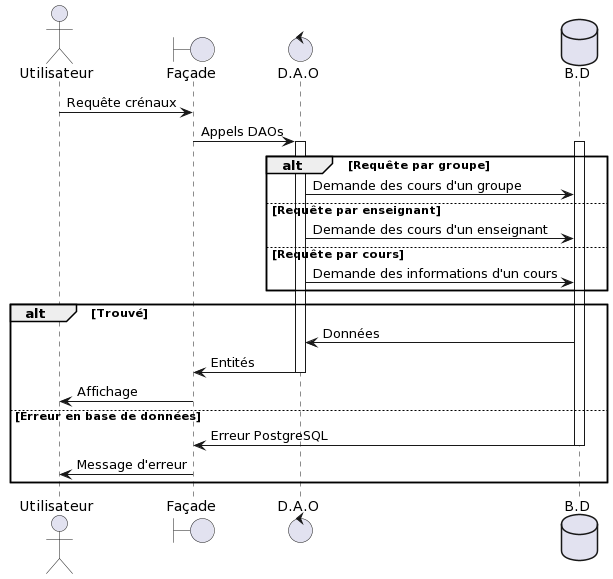
\includegraphics[width=\textwidth]{figures/diag_seq.png}
    \caption[Diagramme de séquence]{Diagramme de séquence lors d'une lecture en base après notification}
    \label{fig:diagseq}
\end{figure}

\section{Entité}
Un élément important a sous-ligner est l'ambivalence d'états que peut avoir une entité, en effet une entité persisté ou non possède deux états
différents, en terme d'implantation ces états sont reflétés avec l'ID.
\begin{figure}[ht]
    \centering
    \includesvg[width=0.5\columnwidth]{figures/stateDiagram.svg}
    \caption[Diagramme d'états]{Diagramme d'états d'une entité}
    \label{fig:diagseq}
\end{figure}


\chapter{Implantation}\label{chap:implantation}
\headepigraph{\emph{\begin{LARGE} We who cut mere stones must always be envisioning cathedrals.\end{LARGE}}}{Crédo des tailleurs de pierre}

En tant d'informaticien, dire que cette partie n'était pas attendue avec impatiente par notre équipe serait un mensonge, aussi étions-nous très heureux de commencer le développement. néanmoins, comme indiquer dans la chronologie, cette étape arriva après quatre itérations, soit plus d'un mois, il s'agit d'un délai important, car au final l'une des étapes les plus importants de la conception et sa confrontation au réel et l'évolution que cela implique. Malgré tout et conscient du temps limite qui nous était imposé, c'est avec enthousiasme que nous avons développé.
Le module Ingénierie logicielle dans sa partie java passe beaucoup de temps as parlé de POO, programmation défensive et design patern, et c'est donc avec une attention toute particulière à ces sujets que nous avons construits notre système.

\section{Entité}
Les entités sont sans doute l'aspect le plus simple de l'implantation, c'est d'ailleurs pour cette raison que l'implantation de ceux-ci a était la première étape dans notre développement. Peu de choses sont as noté de cette partie, sinon bien sur les difficultés rencontrées lors des DAO avec la persistance des entités. L'un des éléments complexe de ces entités est l'intrication entre les $Group$ et les $Etudiant$, cette intrication est bien sûr le reflet de la réalité, implique un choix d'implantation afin d'éviter une redondance d'information qui ne serait
être persister. Le choix final, c'est porter sur les $Group$ qui sont composés d'étudiant.

\section{Facade}\label{section:facade}
La façade est un design patern connue, son but est de fournir une A.P.I afin de simplifier l'usage du modèle et de le découpler du controler.

Dans notre cas, l'usage est multiple :

\begin{enumerate}
    \item \textbf{Formatage :} dans le cadre d'un ajout d'entité, il est nécessaire de fournir des méthodes qui s'assurent de l'uniformité
    du formatage afin d'éviter une interface hétérogène.
    \item \textbf{Exception :} de manière naturelle, notre DAO renvoi un certain nombre d'exceptions et $Optional$. Étant admis qu'une interface
    qui crashe suite à l'échec d'une recherche est inacceptable, il faut traite ces erreurs. Cependant, si on pourrait penser pouvoir traite ces erreurs dans le controleur, ces oubliés la multiplicité $des$ controleurs, aussi la gestion de ces erreurs serait traiter plusieurs fois, ne respectant pas ainsi le principe $DRY$, et provoquant de facto un couplage important entre la DAO et l'IHM. De plus, nous avions pour projet
    d'étendre le nombre Exception, il ne s'agit donc pas d'un problème anodin.
\end{enumerate}

Maintenant des limites sont as sous-ligner, en effet cette façade est de loin le plus gros fichier Java du projet. La raison n'est pas tant
sa complexité, mais sa richesse de surcharge, tant est si bien qu'avec plus de huit-cent lignes la lecture et l'orientation est complexe, rajouter
à ça le patern d'observateur observé, et vous obtenez une facade sans doute trop grosse. Plus important que le nombre de lignes est le scope de
cette facade, c'est facile, il est difficile de trouver une classe sans interaction avec cette facade, ainsi nous nous approchons dangereusement
d'un anti-patern le $god$ $object$. Mais il s'agit d'un choix conscient, motive par la faible échelle de notre projet et la praticité de cette facade.

\section{Interface Homme Machine}
Pendant que les DAOs furent développer en adéquation avec la base de données, la question fut poser de comment pourriez-nous afficher notre application d'emploi du temps autrement que par terminal, la réponse est évidente une interface.

Le sujet ne nous a pas imposer de bibliothèque précise en ce qui concerne l'IHM, donc nos premières déductions, on était peut être une bibliothèque html/java, ou quelque chose de similaire, pour afficher proprement les données dans une page web ou une application standalone.
Au fil du temps les conseils autour de ces questions sont claires, utiliser \emph{JavaFx} pour votre application.
\emph{JavaFx} se fut, et après quelques recherches nous sommes parvenu tout d'abord à trouver une bibliothèque qui réplique un Google Calendar en \emph{JavaFx}, son nom : \emph{CalendarFx}

Une bibliothèque qui s'occupe entièrement d'afficher un planning complet, gérant les évènements à certaines dates et heures, différentes vue sur la semaine ou la journée. Au vue du temps limité dont nous disposions, cette bibliothèque semblait presque trop parfaite.
Donc sur 1 semaine, le travail à été répartis entre nous, quelqu'un s'occupe de continuer la base de données, quelqu'un d'autre s'occupe d'avancer les DAOs en parallèle, et le dernier s'occupait d'intégrer \emph{CalendarFx} dans le projet.

Hors la vision parfaite et utopique que nous a vendu cette bibliothèque s'est vite estompé, l'intégration prenait beaucoup plus de temps que prévu et était bien trop complexe pour très peu d'avancement, on remarqua également qu'elle manquait cruellement de documentation et de ce qui pourrait être utile quant au projet de planning scolaire.

 On essaye donc de continuer et d'intégrer \emph{CalendarFX} au projet juste pour avoir un exemple à montrer lors de la prochaine séances de révision. 
L'avis général a été assez mitigé, donc à partir de là, nous nous sommes concertés et avons décidé de retirer complètement \emph{CalendarFX} du projet, étant donné qu'elle est trop complexe à intégrer pour de simple exemple, ç'aurait été bien plus complexe et problématique de l'intégrer à tout notre système de gestion et de planning.

Finalement, on supprime tout ce qui concerne cette bibliothèque pour repartir de zéro côté IHM, et la semaine qui suit sera surtout un travail de rattraper le retard engendré par \emph{CalendarFX} et de créer notre propre interface de Planning à partir de \emph{JavaFx}.
Concernant la structure de l'interface, on utilise des fichiers XML et CSS pour définir, respectivement, quel composant de \emph{JavaFX}, nous allions utiliser ainsi que leur aspect graphique.
Simplement dit, nous créons des classes intermédiaires pour manipuler facilement notre emploi du temps et afficher son contenu dans une grille (resp. GridPane).

Toute la conception de l'interface à partir de \emph{JavaFx} s'est faite en respectant le paterne \emph{MVC}, comme décrit dans la section Façade\ref{section:facade}, celle-ci sert de pont entre le Modèle et le reste de l'application.
%mvc uml diagram
\begin{figure}[!h]
    \centering
    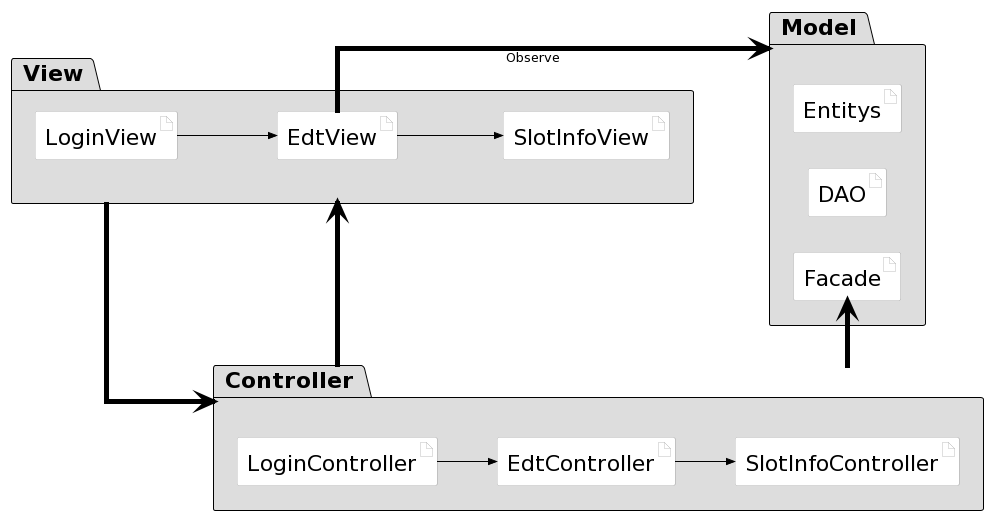
\includegraphics[width=0.7\textwidth]{figures/mvc_pattern.png}
    \caption{Modèle Vue Contrôleur}
    \label{fig:mvc_pattern}
\end{figure}
Donc notre paquet Contrôleur, qui s'occupe de gérer toutes les actions dynamiques de l'interface, communique avec la Façade pour tout ce qui concerne l'ajout, la modification, suppression ou lecture d'un cours, ou d'un emploi du temps.
Puis pour ce qui concerne la Vue, la nuance vient du fait que nous utilisons principalement des fichiers XML, donc pour mimer le fait que la Vue soit actualisée en fonction du Modèle, nous utilisons le paterne \emph{Observateur / Observé} sur le Contrôleur qui observe le Modèle et actualise la Vue en fonction des changements effectués.

Finalement, pour ce qui est des données présentes sur l'emploi du temps, nous avons fait en sorte que des données soient présentes pour le mois de janvier 2023, utile pour les tests et les démonstrations sur des cas plus réels et concrets.

%login view
\begin{figure}[!h]
    \centering
    
\includegraphics[width=0.7\textwidth]{figures/login_view.png}
    \caption{Vue d'Authentification}
    \label{fig:login_view}
\end{figure}
Lorsque l'utilisateur lance l'application, il fera face à la vue d'authentification, il pourra choisir de se connecter comme invité ou bien entrer un e-mail et un mot de passe pour se connecter à son compte. Ce même compte peut être un administrateur, un professeur ou un étudiant. Le procédé est différent s'il s'agit d'un invité.

L'interface du planning s'adapte donc en fonction de l'utilisateur authentifié, par exemple un Administrateur aura la possibilité de voir tous les emplois du temps d'une Promotion spécifique, mais aussi d'ajouter/supprimer/modifier des cours de celle-ci.
%admin view
\begin{figure}[!h]
    \centering
    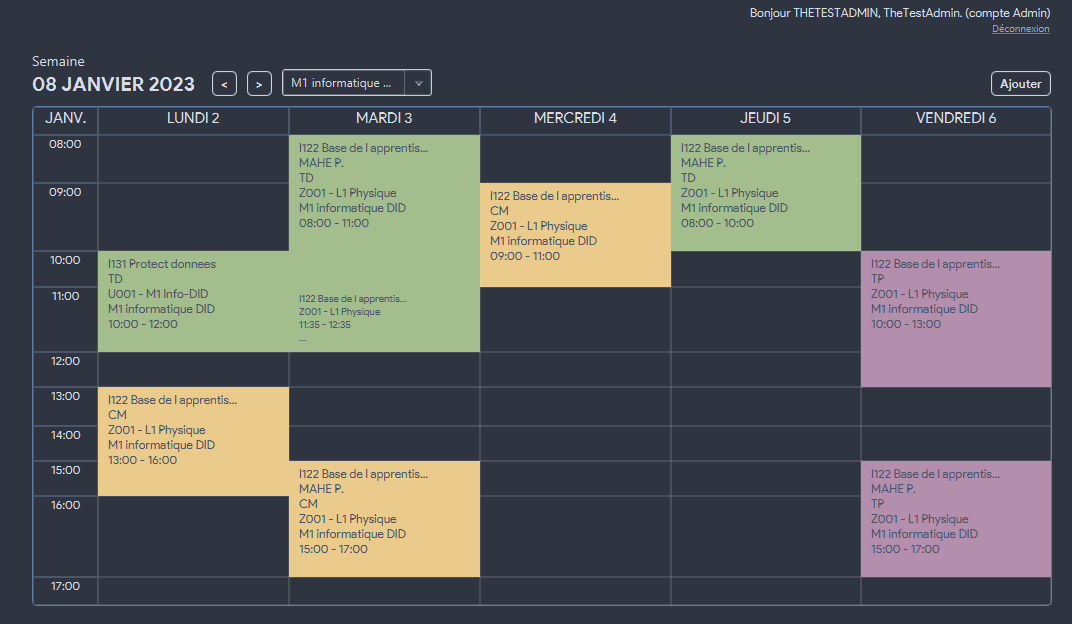
\includegraphics[width=0.7\textwidth]{figures/adminView.png}
    \caption{Emploi du Temps vu par un Administrateur}
    \label{fig:admin_view}
\end{figure}

%student view
\begin{figure}[!h]
    \centering
    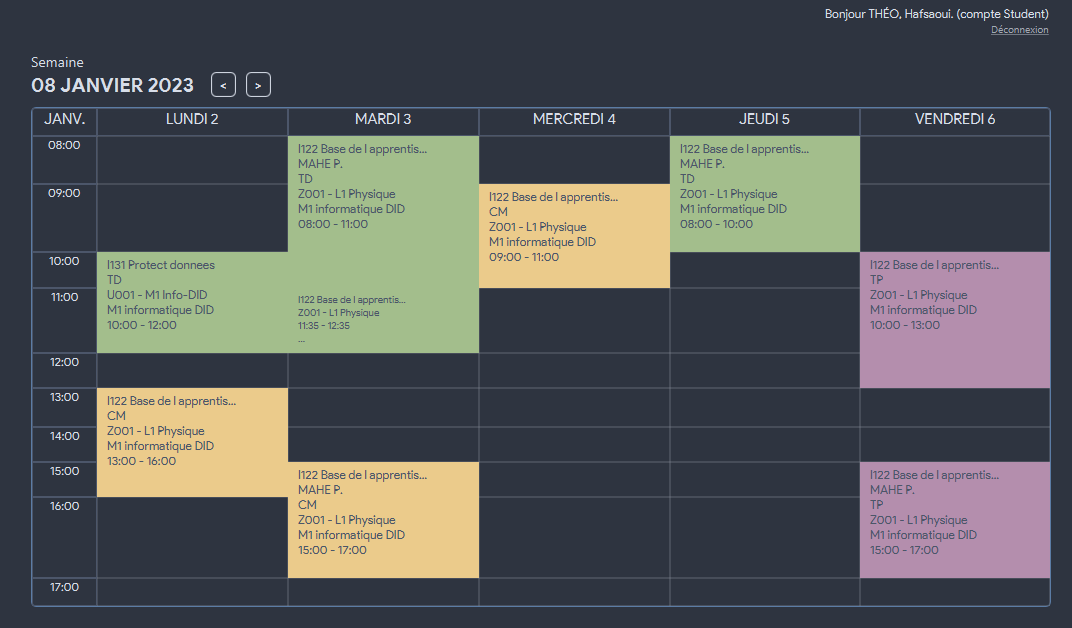
\includegraphics[width=0.7\textwidth]{figures/studentView.png}
    \caption{Emploi du Temps vu par un Étudiant}
    \label{fig:student_view}
\end{figure}
Autre exemple, les étudiants et les professeurs n'ont accès qu'à leurs emplois du temps respectifs, tandis que les invités peuvent uniquement visionner les emplois du temps d'une promotion à sélectionner depuis l'interface.

%cm / td / tp color code photo
\begin{minipage}{0.45\textwidth}
Par défaut, les cours ont un code couleur attribué en fonction du type de cours (c.-à-d. CM, TD, TP, EXAM, RÉUNION, etc).
\end{minipage}
\hspace{0.5cm}
\begin{minipage}{0.45\textwidth}
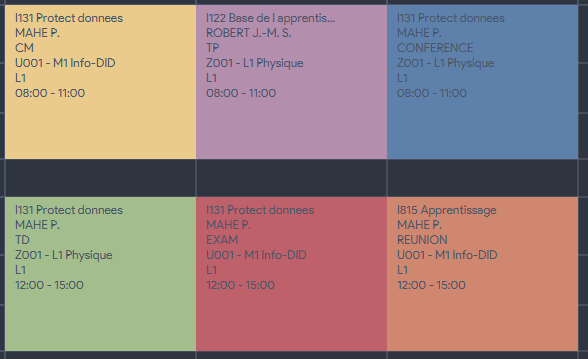
\includegraphics[width=\textwidth]{figures/slotColorCode.png}
\end{minipage}

%slot info panel
\begin{minipage}{0.45\textwidth}
Si la durée de ce cours est inférieur à 2 h, alors certaines informations normalement présentes seront retirées par simple choix de lisibilité, pour remédier aux manques d'informations, il est possible de sélectionner directement le cours en question pour y afficher toutes ces informations (et accessoirement les modifier si on est connecté sur un compte administrateur).


\end{minipage}
\hspace{1.5cm}
\begin{minipage}{0.45\textwidth}
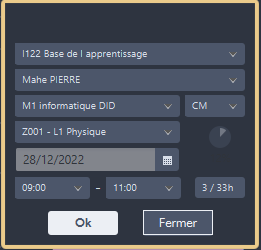
\includegraphics[width=\textwidth]{figures/studentSlotInfoPanel.png}
\vspace{0.5cm}
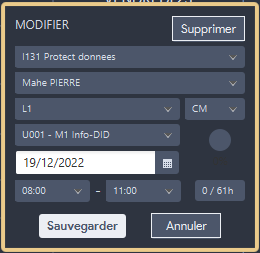
\includegraphics[width=\textwidth]{figures/adminSlotInfoPanel.png}
\vspace{1.5cm}
\end{minipage}
Ce panneau d'informations relatif aux cours permet de facilement afficher toutes les informations d'un cours sélectionné, ou bien pour l'administrateur, de facilement modifier un cours.
Par exemple, admettons un cours a lieu le lundi 5 de 09 h à 10 h pour la promotion M1 DID, si l'administrateur choisit de définir ce cours pour la promotion de L1 Physique, puis sauvegarde ce changement.
La façade du modèle s'occupe d'effectuer les changements sur le dit modèle, puis le Contrôleur en question fait vu d'un changement effectué sur le modèle, et actualise donc l'élément à changer sur l'emploi du temps.
En l'occurrence, le cours de M1 Did, ne serait plus visible pour cette promotion, et serait visible pour la promotion L1 Physique le lundi 5 de 09 h à 10 h.

Le patern \emph{Observateur / Observé} ne notifie l'emploi du temps que des changements qui ont été effectués ainsi que le type du changements à appliquer sur la grille de notre emploi du temps (resp. Ajout / Modification / Suppression).
Autrement dit si je change de promotion le cours du Lundi 5, la Façade effectue l'appel des daos correspondantes pour effectuer le changements en base de données, puis notifie la Façade si les changements sont bien valides, et enfin la Façade notifie tout ces \emph{Observateur} qu'il y a eu un changements sur le cours du Lundi 5, et ce changement est de type \emph{Modification}, puis le contrôleur et la vue font le reste.

\section{Test Unitaire}
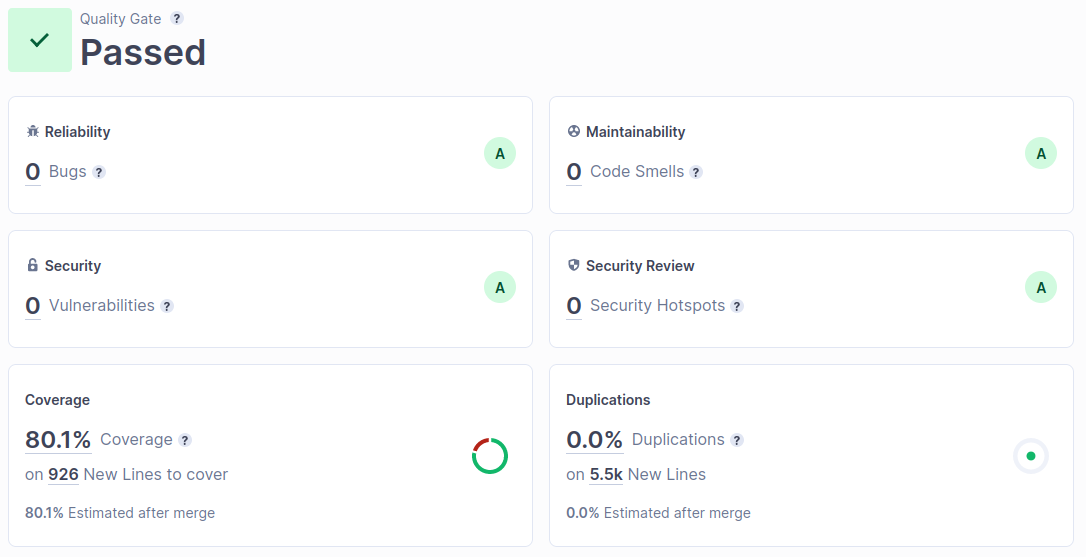
\includegraphics[width=\textwidth]{figures/coverage.png}

Pour commencer cette section, parlons d'un étudiant en Licence d'informatique.
Lors de ces études d'informatique, cet étudiant typique va réaliser un certain nombre de TP dans diverse matière, souvent
sans connexion, où il doit, dans un temps limité, résoudre des courts problèmes. il y a bien des épiphénomènes, les projets,
mais bien trop rare pour avoir des conséquences durable.
Pourquoi cette digression ? C'est pour sous-ligner les raisons de l'absence d'éducation et le rejet envers les test-unitaire des étudiants
n'est pas par fainéantise mais par expérience. En effet pourquoi tester sont code quand le prochain TP auras lieux dans deux jour,
mais surtout pourquoi tester sont code quand le problème appartiens au royaume de des math, un lieu par définition absolument logique est donc predictible.



La raison est simple, la réalité est trop complexe, les individu imprévisible est par conséquent même un logicielle aussi simple que celui d'un emploie du temps
requerrais un travaille gargantuesque pour un résultat incertain. c'est la le domaine de l'ingénierie.
doit ton pour autant abandonner la rigueur. Non.

Heureusement pour nous, la sciences a trouver la solution il y a des siecle, les test empirique. et leur reflet direct en informatique. les test unitaire.
Pour résumer nous croyons sincèrement aux rôle essentielle des test unitaire dans la développement d'un logicielle.  De plus un code tester est un code bien
compartimenter au couplage faible. ces pour ces raison et plein d'autre qu'une des condition essentielle de validation de nos Pull Request(cf Gesttion de projet)était le test systématique est rigoureux des méthodes ajouter.

La conséquence de ce choix est une confiance importante dans notre C.I, après tout un des éléments essentielle au jugement d'une de nos PR était ça capacité as passer tout les test précédant, et as rester dans les frontière de nos objectifs de code coverage.



\section{Gestion de la persistance: Base de données}
Le projet visant à gérer les emplois du temps d'une université, se pose la question de la persistance des données, de leur format, des méthodes d'accès et de l'intégrité. Le sujet du projet, mentionne l'usage d'une base de données, sans plus de détail. Très tôt dans la conception, notre choix s'est porté sur PostgreSQL, et ce pour plusieurs raisons: 
\begin{enumerate}
    \item  Fiabilité  PostgreSQL est connu pour sa fiabilité et sa gestion conformes aux règles ACID, et au centre d'un écosystème mature .
    \item Orienté objet: PostgreSQL est un SGBD relationnel multi-modèle, et comporte des notions d'objet, dont l'héritage, sur lequel on reviendra en détail.
    \item Types complexes: PostgreSQL gère des types complexes et dispose de types temporels intégrés, notamment des intervalles de temps.
    \item Expérience passée: Nous avons, au cours de notre cursus, déjà été amenés à travailler avec cet outil. 
\end{enumerate}

La modélisation et particulièrement le \crtlnameref{fig:diagstat} nous ont permis de dégager des multiples relations entre acteurs.
En somme, la donnée d'un cours peut se résumer en une phrase:

\begin{quote}
    Le vendredi 25 novembre 2021 \textit{de neuf heures à midi}, les étudiants du \textit{Master 1 Informatique} assistent à  une séance de \textit{travaux dirigés}, dispensée par \textit{MM. \bsc{Mallofre} et \bsc{Loiseau}} dans le cadre du module \textit{projet collaboratif (I143)}, en salle \textit{U.001}.
\end{quote}
%<Remplacer par image?>
Les éléments en \textit{italique} caractérisent ce que l'on a ainsi baptisé créneau (\textit{slot}) tout au long de ce projet. 
Nous avons en outre choisi de n'allouer qu'une seule salle à un créneau. 

PostgreSQL gère les intervalles de temps. Cela nous permet, en pratique, de contrôler la bonne cohérence des données sans nous encombrer de détails techniques. 
Nous nous servons de cette facilité afin de s'assurer que deux plages horaires ne se chevauchent pas dès l'insertion. 

À l'aide de déclencheurs (triggers) nous nous assurons en outre que ces contraintes sont aussi respectés pour les groupes et les enseignants concernés par les cours, avant toute insertion ou mise à jour. 

Enfin, afin de faciliter la gestion de l'authentification, on a recours à l'héritage de tables, qui nous permet d'obtenir le rôle et les informations d'un utilisateur à l'aide d'une simple requête. 

Finalement, on a obtenu le schéma suivant:
\begin{figure}[h]
    \centering
    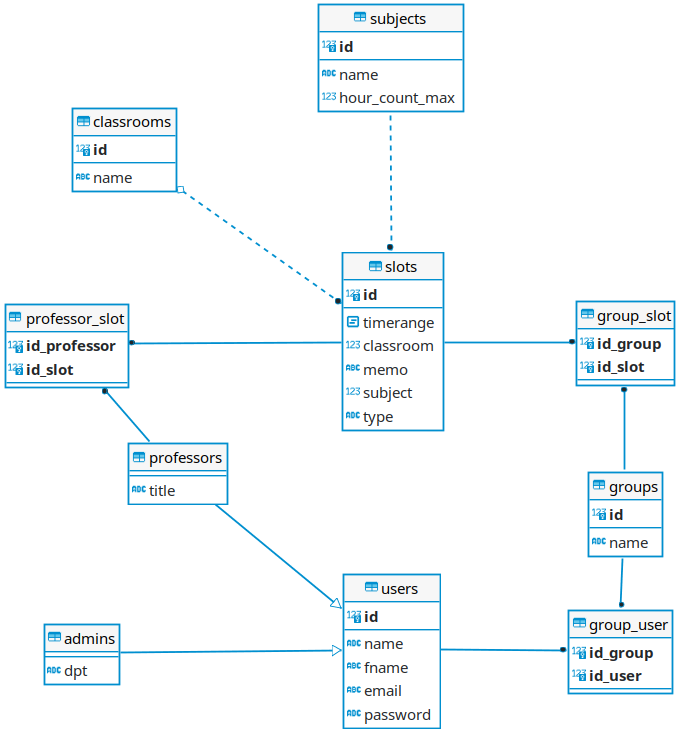
\includegraphics[width=0.5\textwidth]{figures/diagdb.png}
    \caption[Schéma de la B.D.]{Modèle entité relation simplfié de la base de données}
    \label{fig:schemadb}
\end{figure}

Afin de pouvoir accéder à notre base de données en java, nous utilisons le pilote JDBC approprié. Nous avons recours à un agrégateur de connexions \emph{(connection pool)}, qui nous permet de gérer les échanges à la base de données de façon efficace. Il permet en outre de gérer le cas d'une fuite de connexion (si une connexion à la base n'est pas fermée une fois le transfert terminé), ou d'une connexion interrompue (notamment le cas lorsque la base se trouve à distance). 

Afin de segmenter les responsabilités dans notre application, nous utilisons une couche de DAO (Data Access Objects ) qui gère les erreurs, l'instanciation et la persistance en lien avec la base. Lors de la persistance en base, celle-ci génère et nous fournit un identifiant unique, que l'on enregistre dans les entités. 





\section {Intégration continue}

Afin de tester notre code convenablement sans les aléas des environnements des uns et des autres, nous avons jugé utile d'intégrer un système de contrôle de notre code avant son intégration au sein du projet. Des outils, comme Sonar, que nous avons adopté permettent ainsi de contrôler la qualité du code, sa robustesse, d'identifier des failles et les éventuels fragments qui ne seraient pas testés. 

Pour ce faire, la seule solution qui permet un contrôle effectif consiste à contrôler le code que les tests exécutent. C'est le rôle de JaCoCo (Java Code Coverage) qui va ainsi permettre de dégager trois indicateurs principaux : 

\begin{enumerate}
\item Le taux de couverture linéaire, qui mesure la quantité de code  exécuté lors des tests par rapport à la masse du projet. Une règle de bonne pratique consiste à viser un taux situé entre 60 et 80~\%. C'est à ce taux que l'on fait référence le plus souvent. 
\item La couverture conditionnelle (branch coverage), qui vérifie que tous les cas soient testés lors d'une décision. C'est le cas des boucles et rupture de séquences (if, else, while)
\item La complexité cyclomatique qui estime le nombre de décisions prise par un fragment de code donné. 
\end{enumerate}

Il nous faut donc s'assurer que l'agent s'exécute lors des vérifications et que les résultats soient remontés à Sonar, ce qui n'est pas sans quelques déconvenues.

L'exécution se déroule sur une machine mise à disposition par Github, ce qui nous impose d'installer un serveur PostgreSQL lors des vérifications. L'utilisation d'un container docker s'est avérée trop complexe en raison de la multiplicité des acteurs en présence.
%
\chapter{Gestion de projet}\label{chap:gestProjet}
\headepigraph{\emph{\begin{huge}Responding to change\end{huge} over following a plan}}{Agile Manifesto}



Le projet a été réaliser dans un contexte agile, plus spécifiquement avec le framework \texttt{Scrum}.
Scrum est une application des méthodes agile, comme peut l'être aussi l'\texttt{eXtreme programming}, néanmoins cette méthode
se concentre sur l'idée d'itération ou de sprint. Un sprint est une unité de temps arbitraire (un jour/une semaine/un mois) où l'on
se fixe pour objectif de réaliser un nombre $N$ de User Story, ce nombre dépend de la difficulté, de la priorité et le niveau de
risque. l'idée principale étant de mesurer la capacité de travail de l'équipe afin de mieux prévoir et trouver les goulots
d'étranglements. Néanmoins, même si de nombreuse méthode et idées de \texttt{Scrum} était adaptée et bienvenue, ce n'était malheureusement pas le cas des sprints.



En effet, les sprints partent d'un postulat, la comparaison entre Unité de temps similaire, néanmoins ce postulat n'est 
pas raisonnable dans le contexte du premier semestre du M1. D'abord, car ce semestre est variable en temps libre avec des périodes de
vacances, des périodes de cours et des séminaires d'une semaine. Mais surtout, ce Semestre est composé de 6 autres matières, ou 3 d'entre elles demandant un projet ou un équivalent, à de diverses échéances. Il est dès lors impossible de comparer le travail fourni par l'équipe sur deux semaines différentes.



Par conséquent, le choix de l'équipe a été de consigner et prévoir par itération, mais aussi et \emph{surtout} de travailler de
manière \emph{continue} et \emph{incremental} en acceptant la nécessiter du changement.

\section{Chronologie}
\begin{enumerate}[label=\textbf{Itération~n\kern-0.5bp\textsuperscript{o}~\arabic*:},start=0]
    
    %iteration 0
    \item La première itération avait trois objectifs :
    \begin{enumerate}
        \item [\ding{51}]Choisir et mettre en place l'environnement de travail \LaTeX, le choix du workflow \texttt{git} avec github~actions et enfin la mise en place des outils de communication.
        \item [\ding{51}]Définir des acteurs principaux de notre système et interviews pour mieux les comprendre.
        \item [\ding{51}]Établir une veille d'information sur les solutions déjà existantes.
    \end{enumerate}
    
    %iteration 1
    \item La deuxième itération est un peu spéciale, en effet celle-ci as été marquer par une absence de cours.
    par conséquent le chois fait fut celui d'une continuation travaille de l'inception.
    \begin{enumerate}
        \item [\ding{51}]Scission des UC, à partir des interviews de la précédente Itérations
    \end{enumerate}
    
    %iteration 2
    \item La troisième itération fut très court, 4 jours, par conséquent la majorité des modifications provient du feedback de \texttt{Sopra}
    \begin{enumerate}
        \item []Correction des UC à partir des remarques de \texttt{Sopra}
        \item [\ding{51}]Première version d'un diagramme de classe (\emph{information view})
        \item [\ding{51}] Réalisation d'une \emph{Buisness view}
    \end{enumerate}

    %iteration 3
    \item La quatrième itération fut le moment de la création des \textit{User Story}, et de leur chiffrage
    il s'agissait aussi du moment de la création du diagramme de kanban sur github.
    \begin{enumerate}
        \item [\ding{51}] User story et chiffrage
        \item [\ding{51}] Création du diagramme de kanban
    \end{enumerate}

    %iteration 4
    \item La cinquième itération est le moment où le développement de l'application a vraiment commencer.
    avec le début de l'implantation des classes avec leur package respectif. avec comme toujours,
    les tests.
    il s'agit aussi du début des tests en condition réelle de l'I.C, et de nos premiers pas avec le workflow \texttt{Github}
    \begin{enumerate}
        \item [\ding{51}] Implantation classe des packages \texttt{User} et \texttt{Slot}
        \item [\ding{51}] Mise en pratique du workflow \texttt{Github}
    \end{enumerate}

    %iteration 5
    \item La sixième itération fut centrée autour de la Base de donnes, un travaille précédant avait été
    fait en termes de conception, mais l'implantation fut complexe, c'est aussi par conséquent le début du développement
    de la DAO.
    \begin{enumerate}
        \item [\ding{51}] Première version de la base de données
        \item [\ding{51}] Commencement du travaille sur la DAO
    \end{enumerate}

    %iteration 6
    \item La septième itération est la prolongation directe de la cinquième avec un travaille sur la DAO
    est sur la Base de Données, c'est aussi le moment où fassent a l'impératif de temps important une étude
    sur la viabilité du framwork \emph{CalendarFx} as été .
    \begin{enumerate}
        \item [\ding{51}] Travaille sur la base de donnes
        \item [\ding{51}] Continuation du travaille sur les DAO
        \item [\ding{51}] Etude des choix pour la GUI
    \end{enumerate}

        %iteration 7
    \item La huitième itération est l'itération de la première iHM, avec l'abandon de \emph{CalendarFX} est l'adoption
    de \emph{JavaFX}, avec aussi des modifications sur la DAO avec le choix de \emph{Hikari} pour la gestion des pools
    de connections.
    \begin{enumerate}
        \item [\ding{51}] Première IHM
        \item [\ding{51}] Continuation du travaille sur les DAO avec Hikari
        \item []  Fin du travaille sur la base de donnes
    \end{enumerate}
    
    %iteration 8
    \item La neuvième itération est la première pendant les vacances, pas sans contrainte, mais un peu plus
    flexible. c'est le moment où les DAO et la base de donne furent terminées, avec une première tentative
    de connexion entre les deux avec une façade. Néanmoins, cette période fut aussi celle d'un bug sur
    l'Intégration Continue.
    \begin{enumerate}
        \item [\ding{51}] amélioration de IHM
        \item [\ding{51}] fin du travaille sur les DAO et la base de donnée
        \item [\ding{51}] Implantation de US1
    \end{enumerate}
    
        %iteration 9
    \item La Dixième itération as aussi eu lieux pendant les vacances, elle avait pour objectif de préparer la
    réalisations de \textbf{toute} les US la semaine suivant
    \begin{enumerate}
        \item [\ding{51}] fix de I.C
        \item [\ding{51}] continuation travaille d'implantation avec les US2 US3 US4
        US5
    \end{enumerate}
    
            %iteration 9
    \item La Onzième et dernière itération qui avait évidement pour objectif de finir ce projet
    \begin{enumerate}
        \item [\ding{51}] rédaction rapport et manuel
        \item [\ding{51}] Fin de de l'implantation avec la US6
    \end{enumerate}
    \begin{center}
        \begin{Large}
            FIN DU PROJET\\9 Janvier 2023
        \end{Large}
    \end{center}
    
    
\end{enumerate}
\section{GitHub flow}
Le choix d'un workflow ou manière de travail est un élément essentiel à toute gestion de projet. Chacun des membres de notre équipe
a vécu un projet avec une répartition du travail arbitraire, individuel et en parallèle avec une réunion du travail catastrophique à la fin.



Bien sûr, un fix simple à ce problème est \texttt{Git}, néanmoins il ne s'agit que d'un outil et comme tous les outil, la manière
de l'utiliser est au moins aussi, sinon plus, importante que l'outil lui-même.
Nous avons, en cours, étudié l'un des workflow les plus connus, le \emph{feature flow}, ce workflow, bien qu'efficace et familier de 
la majorité de notre équipe, présente une faiblesse ennuyante. Il est en effet difficile de lire le travail des autres.
D'abord un développeur peut travailler sur plusieurs Feature, donc branche, et ensuite et surtout le travail peut être
merger de manière unilatérale et sans vérification de toute l'équipe.

Le GitHub flow est une solution à ces problèmes, principalement utiliser sur les dépôts Open Source de Github, ce workflow est particulièrement adapté à un travail en groupe, puisqu'il est la base de projet avec plusieurs milliers de contributeurs.
Bien sûr, notre groupe n'a pas besoin d'une telle scalability, non, l'intérêt principal qui nous à pousser vers ce choix est la 
sécurité et la communication qu'ils entraînent. Ce workflow est en effet caractérisée par une certaine rigidité des branches, cette
rigidité découle de l'importance des \emph{pull request}(PR).


Ces \emph{PR} sont un véritable hub de discussion du 
travail en cours, avec des fonctionnalités comme les draft, les commentaires, le support de markdown et enfin et surtout des \emph{code review}. Des review avec un twist, puisque que nous avons décidé que toutes les branches seront accepter à \textbf{l'unanimité},
pour rendre les choses plus claire, ci-dessous un exemple du workflow.
\subsection{description du workflow}
\begin{minipage}{0.5\textwidth}
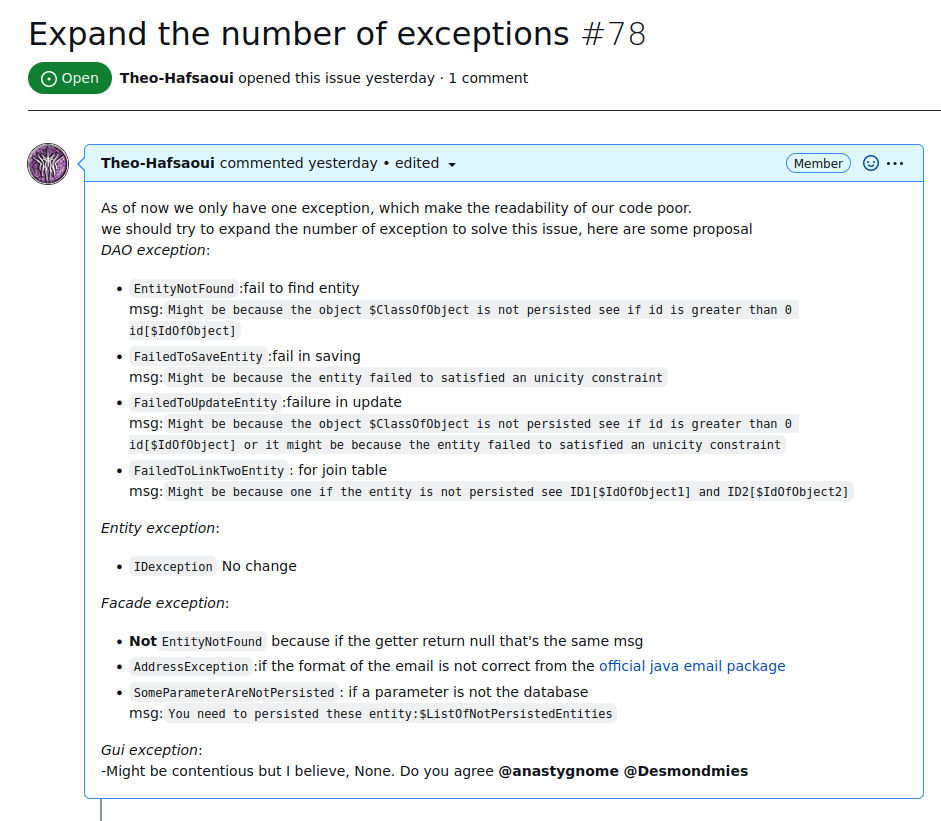
\includegraphics[width=\textwidth]{figures/issue.png}
\end{minipage}
\begin{minipage}{0.5\textwidth}
\vspace{0.5cm}\\
\underline{Etape 1:}La première étape de notre méthode de travail est l'ouverture d'une \emph{issue}.
En général cette issue est le résultat d'une réunion est et toujours accompagner par plusieurs autres.
Certaines issues sont des \emph{meta-}issue, des issues tellement grosse qu'il serait dangereux et surtout bloquant
de les réalisées en une seule Pull Request. Par conséquent, ces Issues ne sont réalisées que si un autre nombre d'issues sont
résolue auparavant, github permet d'ailleurs de le faire automatiquement
\vspace{2.5cm}\\
\end{minipage}

\begin{minipage}{0.5\textwidth}
\underline{Etape 2:}La deuxième étape est celle de la communication, en effet l'issue n'est qu'une proposition amenée naturellement à évoluer en fonction des remarques et contraintes des membres de l'équipe. On retrouve en général une décomposition du travaille, sous forme de check-liste
et parfois des diagrammes UML pour enlever les ambiguïtés, ces diagrammes sont d'ailleurs toujours présents sur les issues des User Story
\end{minipage}
\begin{minipage}{0.5\textwidth}
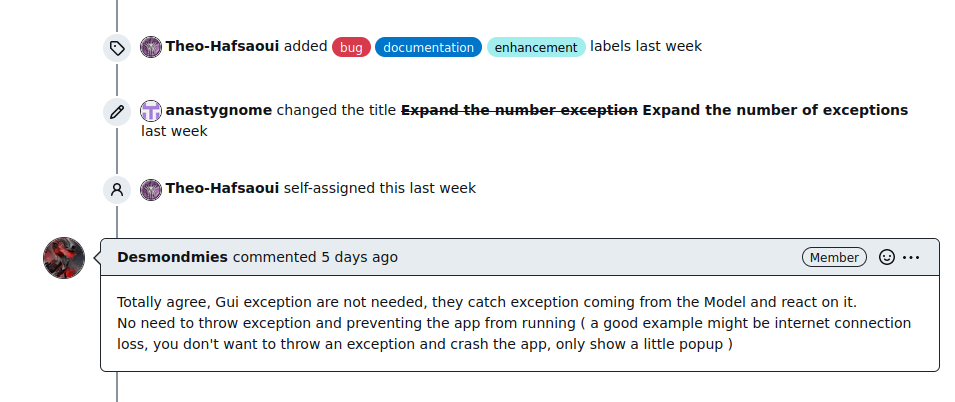
\includegraphics[width=\textwidth]{figures/comment.png}

\end{minipage}

\begin{minipage}{0.5\textwidth}
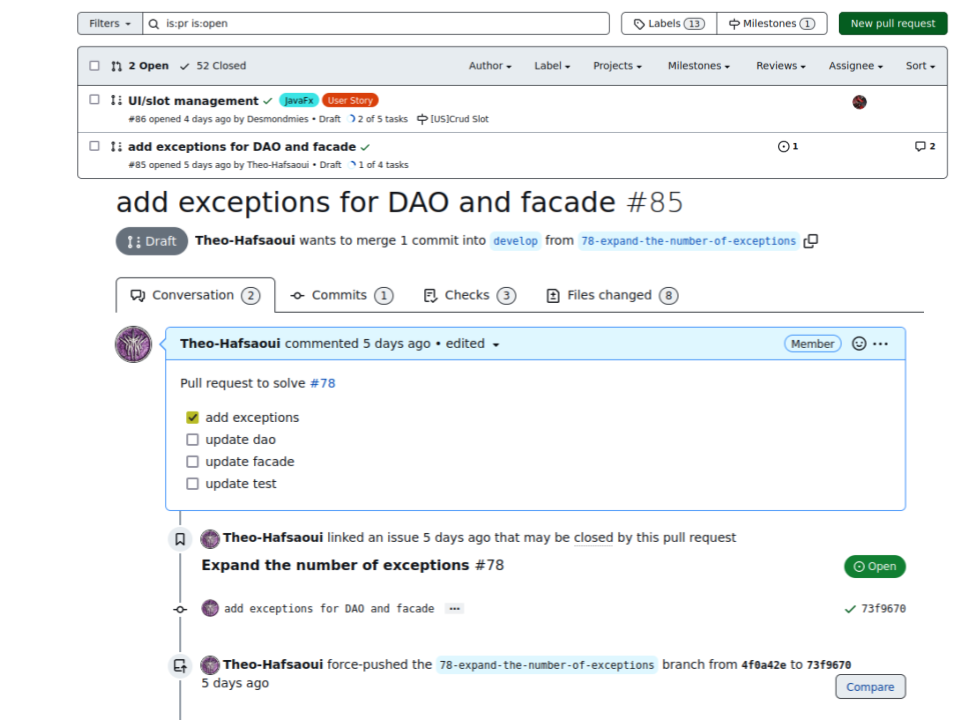
\includegraphics[width=\textwidth]{figures/OpenPr.png}
\end{minipage}
\begin{minipage}{0.5\textwidth}
\vspace{2.5cm}\\
\underline{Etape 3:}La troisième étapes est l'ouverture de la pull request, c'est là aussi un hub de discussion, mais d'une nature différente de
l'issue. Là où la priorité des discussions d'une issue sont de lever les ambiguïtés et définir les objectifs, les Pull Request elle dans leurs
discussions se concentrent sur l'aspect technique, performance, lisibilité, documentation et bien sûr les tests unitaire.
\end{minipage}

\begin{minipage}{0.5\textwidth}
\underline{Etape 4:}La quatrième étape est la review, en effet les discussions précédentes étaient sur une Pull Request en mode \emph{Draft}, c'est-à-dire qu'il était sur un travail en cours. La review est différente, car si les discussions sur le draft sont facultatives, la review est absolument
obligatoire. Cette review peut finir par deux résultats différents. Le premier résultat est bien sûr, l'acceptation de la PR par toutes les membres
de l'équipe, il s'agit du résultat le plus commun grâce aux discussions au moment des rétrospectives et le travaille de fond réalisé dans les issues.
Le Deuxième résultat assez commun lui aussi est la demande de modification, les raisons sont diverses, mais en général il s'agit d'un problème de cohérence avec le reste du code ou une optimisation.
\end{minipage}
\begin{minipage}{0.5\textwidth}
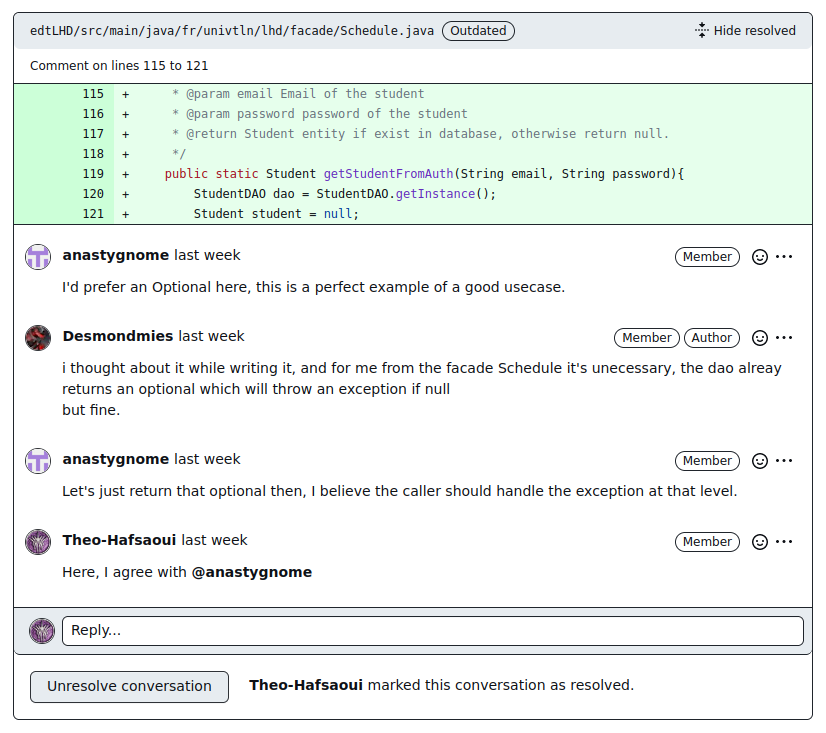
\includegraphics[width=\textwidth]{figures/review.png}
\end{minipage}

\begin{center}
    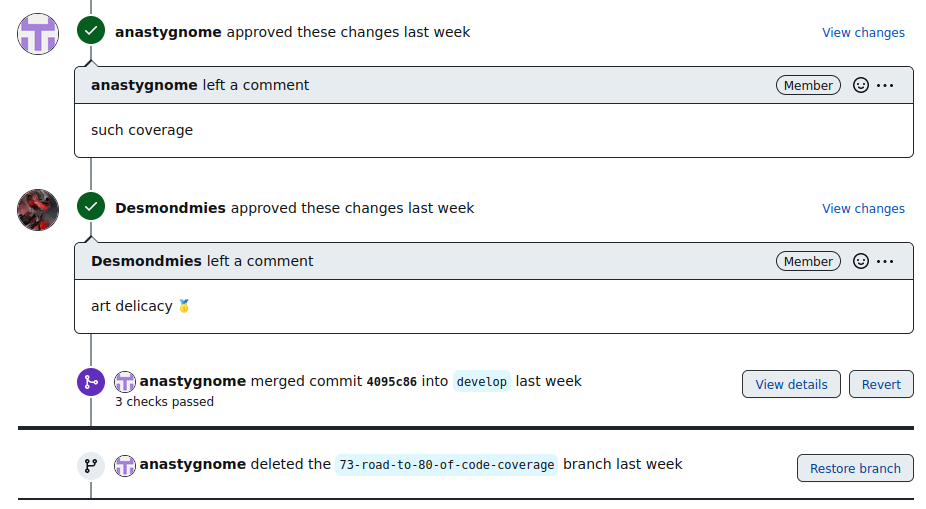
\includegraphics[width=\textwidth]{figures/end.png}
\end{center}


La dernière étape est bien sûr l'acceptation de la PR et le rebase, avec en général un squash, sûr développe.


Certains points sont tout de même à noter :
\begin{itemize}
    \item \emph{Anglais}: Le choix de la langue sur Github n'est pas un choix anodin, mais une véritable volonté de professionnaliser notre projet. Après tout l'anglais n'est pour aucun d'entre nous notre langue natale, un effort de concisions des idées étaient donc nécessaires pour pouvoir communiquer dans nos Pull request
    \item \emph{Github} Le choix de la plateforme de Microsoft découle de l'intégration entre les différentes briques de notre projet,
    par exemple la création d'une issue crée un ticket dans le kanban et sa résolution faisait glisser ce ticket dans la bonne colonne.
\end{itemize}


\subsection{limite}
Comme évoquait précédemment ce workflow offre de nombreux avantages, mais il n'est pas sans inconvénients.
\begin{itemize}
    \item D'abord il s'agit d'une méthode lourde. En effet, chaque PR est soumise à la disponibilité des membres de l'équipe,
    par conséquent l'indisponibilité paralyse l'avancement dans le cas d'une PR critique.
    \item Il ne s'agit pas d'une faiblesse du workflow github, en général, mais dû notre spécifiquement.
    en effet, dans un souci de lisibilité, chaque PR ou presque à était squash, à un ou plusieurs commits.
    rendant la lecture de l'historique plus facile, mais surtout fausse. ce qui peut donner une vision biaisée de l'historique.
\end{itemize}
\newpage
\section{Kanban}
\begin{figure}[h!]
    \centering
    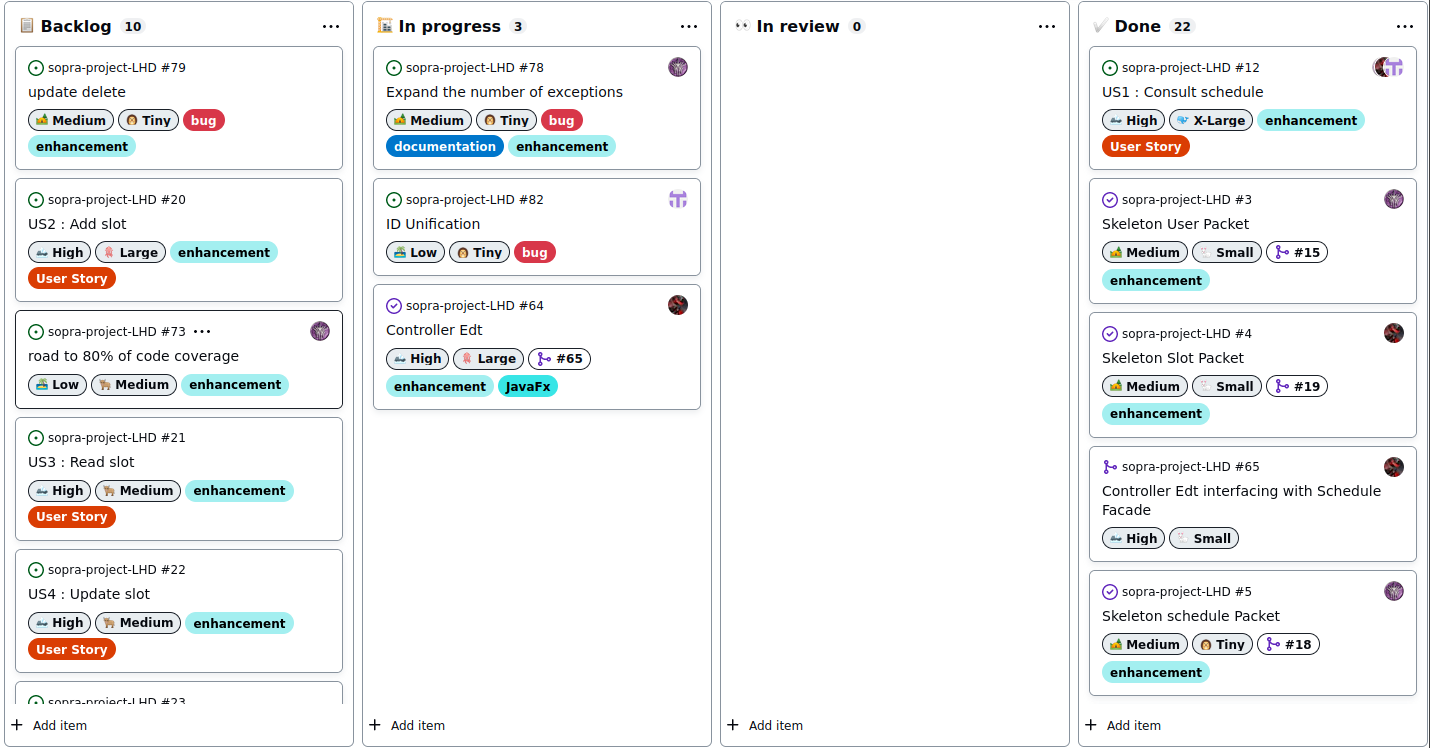
\includegraphics[width=0.9\linewidth]{figures/kanban.png}
\end{figure}
\hspace{2cm}

Bien sûr, un workflow n'est pas suffisant, la production d'un logiciel est un art complexe, particulièrement lorsque
l'on souhaite paralléliser les tâches. À cette fin, c'est naturellement que nous nous sommes dirigés vers un autre outil que \texttt{Github} propose le diagramme de kanban.
\hspace{1cm}



\textbf{Le principe: }Ce diagramme se décompose en trois grandes parties.\underline{Todo}(A faire),\underline{In progress}(en cours),\underline{Done}(fait).Par exemple, si on reprend notre workflow vu précédemment, l'ouverture d'une issue est la création d'un ticket qui va dans la colonne Todo(Backlog car nous utilisons \texttt{Scrum}). l'ouverture d'une PR nous amènent directement dans
la colonne In Progress et enfin la validation de la PR fini dans la colonne Done.

Simple et souvent associer à \texttt{Scrum} il est néanmoins très différent dans son approche du temps, qui ici est continue au contraire
de \texttt{Scrum} qui lui à une approche itérative. Cette différence est sans doute pour nous l'intérêt essentiel de ce diagramme.
En effet, comme expliqué dans l'introduction de ce chapitre, suite aux multiples contraintes de ce semestre, le choix de notre équipe
à était d'abandonner le format itératif de \texttt{Scrum} pour une version continue. Par conséquent, un risque important
était le manque de vision global du projet, après tout, il s'agit d'une des forces de \texttt{Scrum} avec sa capacité de prévision. Kanban est une solution directe à ce problème, s'il n'est pas aussi efficace pour prédire, il est absolument parfait
pour s'assurer de la cohérence et de la synchronicité du travail de chacun des membres de l'équipe.

Commencer par le Kanban est néanmoins légèrement mensonger, car il est au final le résultat du travail réalisé sur le backlog et
la sprinte table. Ces deux tableaux, on était réalisés à l'initiative des intervenants et fut indispensable dans la priorisation des tickets, ce fut aussi pour l'équipe l'occasion de confronter nos prévisions, une étape essentielle, car avec l'abandon des itérations notre
capacité de prédiction devait être le plus aiguisée possible.

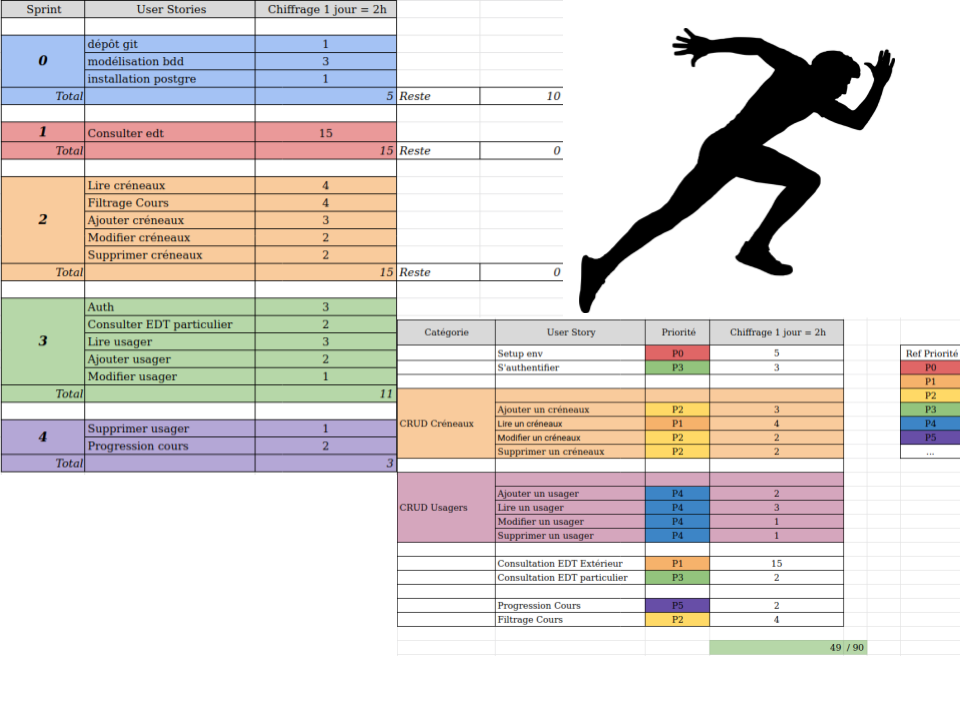
\includegraphics[width=0.9\linewidth]{figures/sprint.png}

Néanmoins, malgré tout les avantages de ces tableaux, ceci était par définition statique et lourd à entretenir. Heureusement pour nous, github propose une solution.
Peut-être ne l'avons-nous pas assez souligné précédemment, mais le passage d'une colonne à l'autre est absolument automatique, ce qui ici est
une solution à notre problème de tableaux statique, et en effet dans le reste du projet, nous utilisons le Kanban \emph{mais} avec différent
filtre, en effet github permet d'appliquer des labels de taille et de priorité pour ensuite les trier par ces paramètres.
Devant ces features, il à donc était naturelle pour nous de complètement basculer sur Github, mais sans abandonner les sprints Table juste
en les convertissant de manière naturelle dans notre workflow.

\begin{center}
    

\begin{minipage}{0.4\textwidth}

\begin{center}
    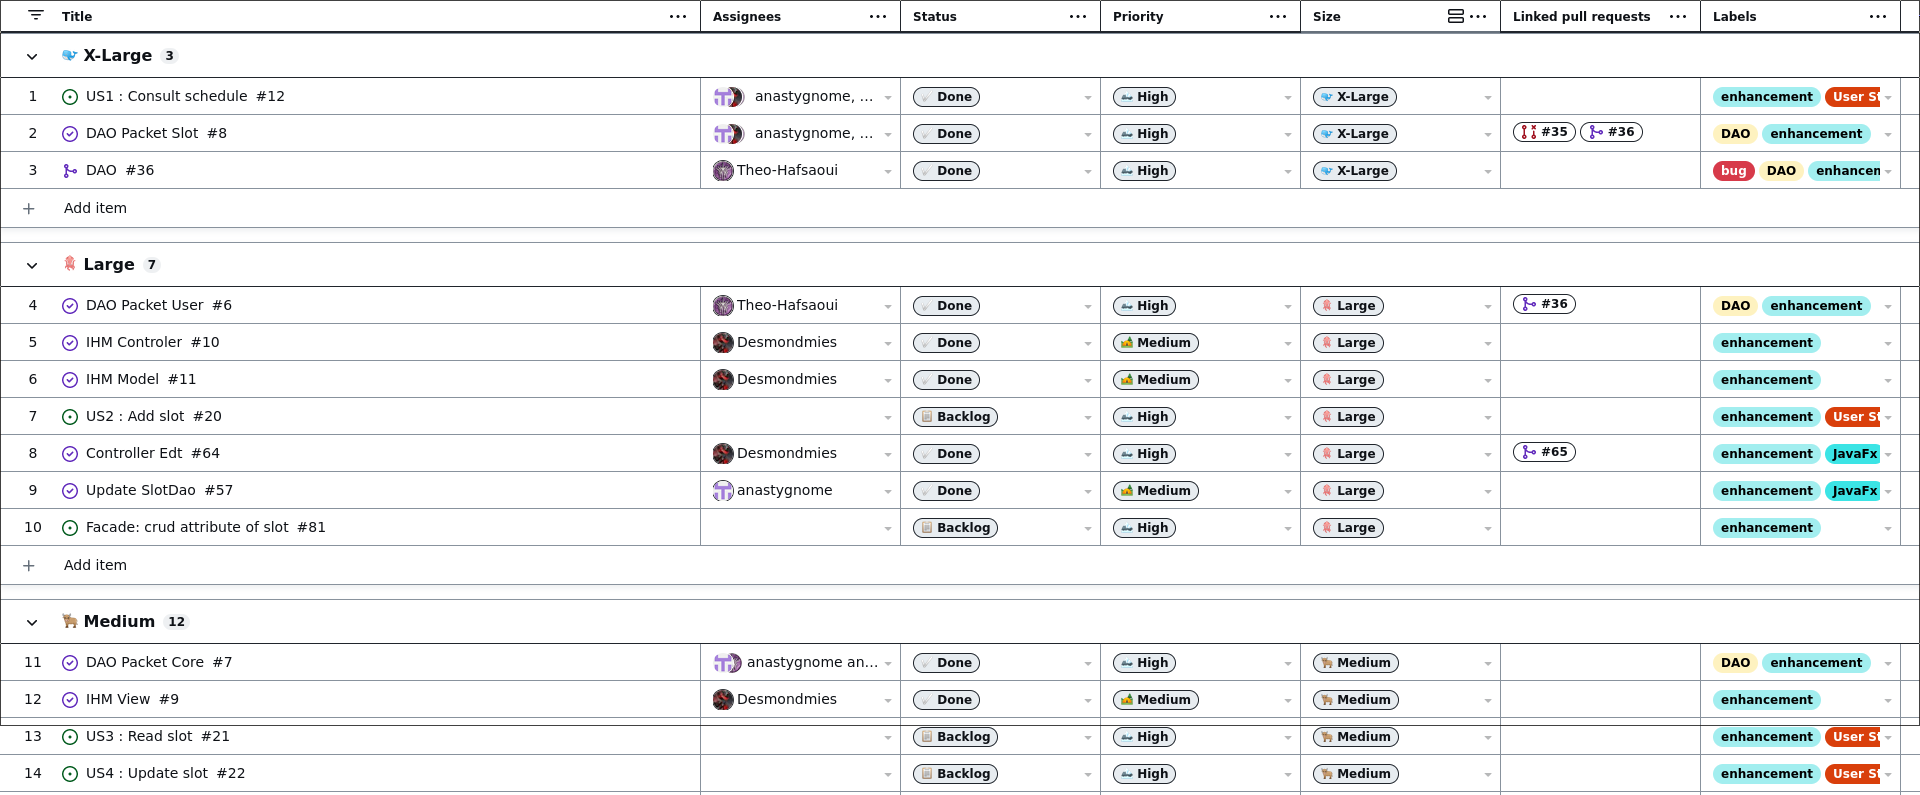
\includegraphics[width=\textwidth]{figures/size.png}
\end{center}

\end{minipage}
\begin{minipage}{0.4\textwidth}

\begin{center}
    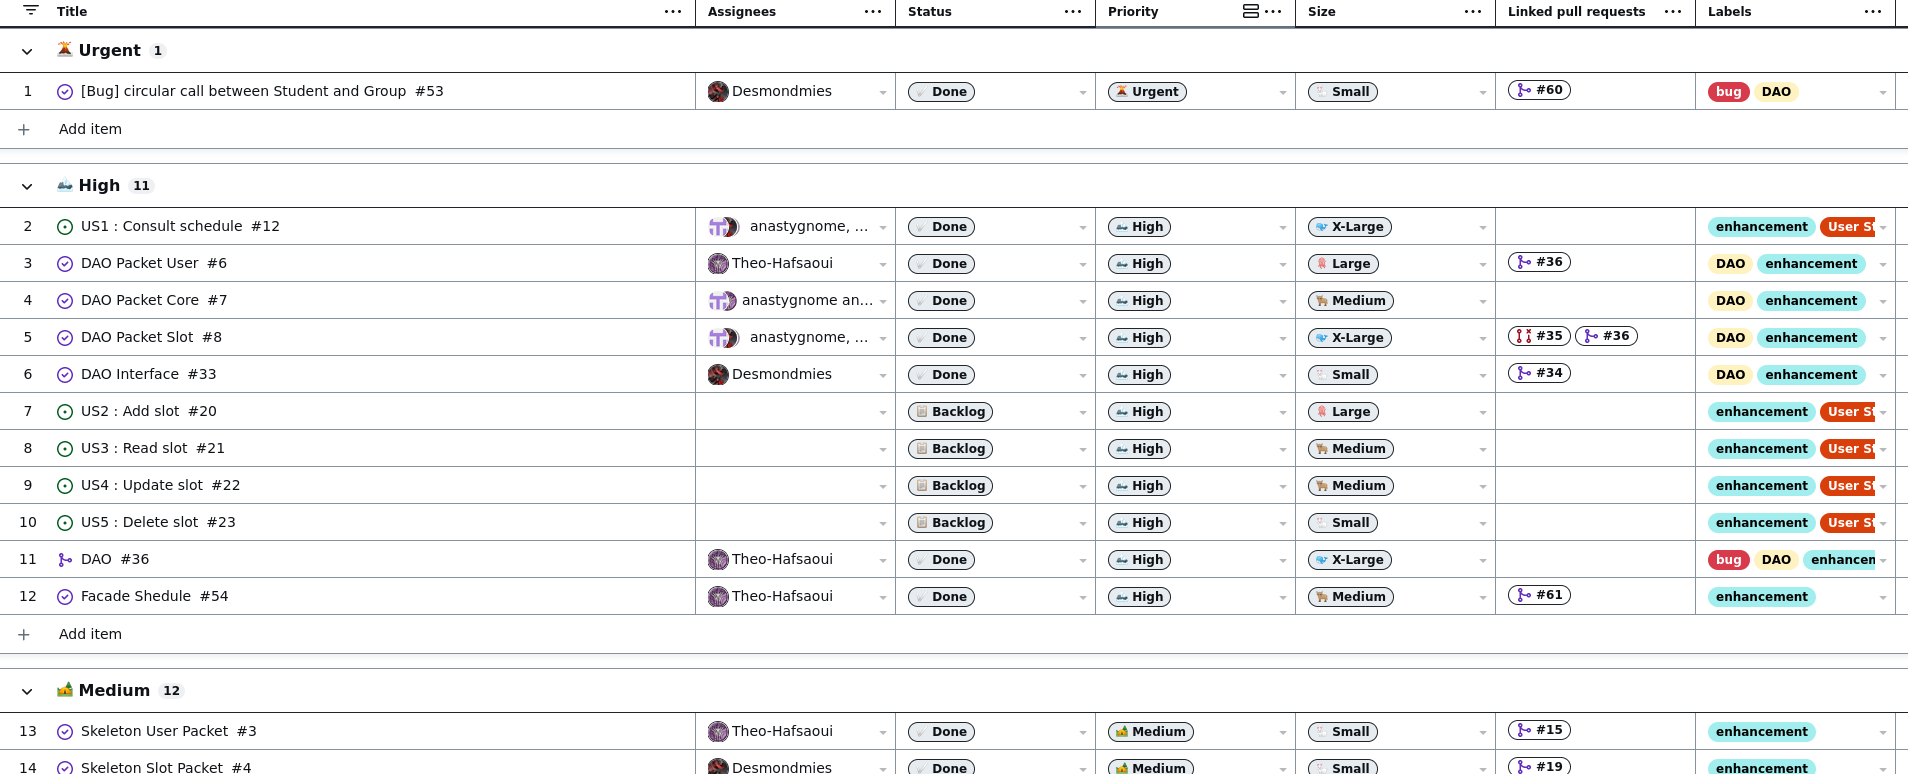
\includegraphics[width=\textwidth]{figures/urgency.png}
\end{center}

\end{minipage}

\end{center}





\section{Analyse \& conclusion}

Juger de la gestion d'un projet, est une tâche presque impossible tant les raisons du succès d'un projet
sont difficile à cerner. D'ailleurs la définition de succès est profondément subjective, particulièrement
pour nous qui n'avons aucun clients à satisfaire, par conséquent et en pleine consciences de la subjectivité
de cette affirmation, nous déclarons que ce projet est un succès.


Maintenant dire que ce projet est un un succès ne nous avance pas beaucoup sur l'analyse de notre gestion de
projet. Certain pourrais même dire qu'un échec aurais rendu l'analyse plus simple est nous aurais éviter une
exposition inutile au biais du survivant. Néanmoins nous croyons que nos expérience passer nous permette une
certaine objectivité sur la gestion du projet et sur ces forces.
\begin{enumerate}
	\item  \textbf{Communication}: Il nous semble que la force de notre gestion de projet se trouve dans
	l'importance accorder à la communication entre ces membres.
	L'exemple le plus frappant de ce choix est sans doutes les code reviews, et l'accord unanime qu'exigent
	une PR, un choix plus que rare et qui découle directement de nos expériences des projets passés ou
	la racine de nos soucis était la communication.

	\item \textbf{Continue}: comme dit dans l'introduction de ce chapitre l'un des choix fait dans l'inception du projet est l'abandon de l'aspect itératif de \texttt{Scrum} au profit d'une vision plus continue. ce choix directement traduit	par le diagramme de kanban, ce diagramme nous as permis une grande flexibilité et agilité sur notre capacité a répondre au changement. Ce qui par exemple nous as permis de rattraper notre retard sur l'IHM après le choix de calendarFX
\end{enumerate}

Néanmoins certaines limites sont à notés de ces points forts. D'abord la communication est une épée a double tranchant, certes le risque d'erreur, d'incompréhension et de duplication du
travaille est réduite mais au détriment d'une forte rigidité et par conséquent d'une lenteur dans l'ajout de nouvelle US. Il nous auras par exemple fallu attendre la dixième itération pour
réaliser la première US. l'intégration Continue bien que à la frontière entre Implantations et notre Gestion de projet, et pourtant une part essentielle de notre manière de
travailler pour ce projet et si les avantages indéniables ont étaient démontrer plus tôt dans ce rapport, cette IC n'est pas sans désavantages dans notre workflow puisque son fonctionnement et
une étapes critiques pour la vision et la fluidité de notre gestion de projet. Ainsi malheureusement pendant 2 semaines suite à des conflits avec PostgresSQL, un poids supplémentaires étaient ressenti dans notre
organisation.

En conclusion, nous nous accordons pour dire que l'aspect le plus intéressant de ce projet est sans doute la gestion de celui-ci et somme très satisfait du résultat et connaissance acquise dans ce projet.

\chapter{Conclusion analyse \& ouverture}
En guise de conclusion, cette aventure de 2 mois nous a inculqués de nombreuses compétences, que ce soit côté \emph{Java} ou côté \emph{Gestion de Projet}.
La découverte de \emph{JavaFX} et la structuration d'un projet complet à plusieurs nous a apporter une réelle plus-value en ce qui concerne \emph{Java}. Enfin grâce à la supervision de \thesupervisor \space durant les différentes semaines dédié au projet et à sa gestion, nous avons concrètement appliquer les principes agiles, cela nous a permis de mieux nous organiser pour les taches à effectuer et terminer le projet dans le délai imposé de 2 mois.
En guise de rétrospective, un projet de cette ampleur aurait pris bien plus de temps et aurait été moins bien organisés sans leur aide.
Comme dit précédemment notre \emph{workflow Github} à également été une décision majeur quant à l'organisation du projet, et réussir à s'en tenir jusqu'au terme du projet est un accomplissant et des compétences acquises en plus pour chacun d'entre nous.
Les seuls point faibles à retenir serait peut être, le début de projet légèrement tardif, ce qui a forcé le gros travail de développement sur la période de fin d'années, en groupe et à distance, ce qui n'est jamais évident à gérer.
Malgré tout nous avons réussi à utiliser les outils à notre porté pour rester dans les temps et rendre un produit fini en adéquation avec la demande client, laissant évidemment possibilités d'améliorer ou changer certains aspects de l'application selon les retours du client.

Comme par exemple des améliorations côté interface :
\begin{enumerate}
	\item \textbf{Message d'erreur}: A l'heure actuel certains messages d'erreur ne sont pas encore affichés par l'interface pour donner un retour direct à l'utilisateur, si une action à provoquer une erreur la plupart du temps il ne se passera rien. L'application continue comme si rien ne c'était passé, une amélioration évidente est de prévenir l'utilisateur du problème actuel, que ce soit un soucis en base de données par exemple l'insertion d'un cours à un créneau indisponible, ou tout simplement la perte de connexion avec la base de données.

	\item \textbf{Rendre l'application parfaitement Responsive}: Un problème majeur lors de l'intégration de \emph{JavaFX}, le fait que l'application devrait être totalement responsive est un chose agréable à avoir pour l'utilisateur. Or actuellement certains cours sont bloquant pour la grille de l'emploi du temps, ce qui rend l'affichage pour de petit écran très complexe voir impossible. La solution idéale serait de rendre l'application compatible Smartphone ainsi que Pc, pour couvrir un large éventail de taille d'écran et donc assurer le côté responsive de l'application.

    \item \textbf{Drag \And Drop}: Un bon point de facilité d'utilisation pour l'administrateur, pouvoir directement glisser les cours sur l'emploi du temps pour rapidement changer leur créneaux ou bien les glisser d'un groupe à l'autre ou d'une semaine à une autre.

    \item \textbf{Multi-Sélection}: Encore un autre point très ergonomique pour l'administrateur, pouvoir sélectionner plusieurs cours, puis effectuer des actions sur chacun d'entre eux, tous les supprimés, modifier des champs, etc.

    \item \textbf{Template}: L'utilisation de template de cours pour faciliter l'ajout répété de cours similaire, par exemple un écran de type de cours préfait, pour permettre à l'administrateur de direction sélectionner un cours pré-rempli et modifier quelques champs pour l'adapter à son besoin, un simple ajout mais qui serait fort utile pour de longue session de gestion.
\end{enumerate}

Certains aspects plus technique quant aux améliorations évoqués pour ce projet sont déjà documentés sur notre \emph{RoadMap} associées.
En outre, ce fut une expérience remplit de concept et de notion rarement traités, une bonne expérience qui nous apportent compétences et connaissances pour la gestion de nos projets futurs ainsi que la structuration d'un projet en prévoyant son ampleur et en chiffrant ses différents aspects afin de le mener à bien dans le temps imparti.

\appendixpage
\appendix

\backmatter
\listoffigures
\newglossaryentry{gls:cha}{name=chobot,description=Lorem}
\newglossaryentry{gls:czi}{name=čížek,description=ipsum}
\newglossaryentry{gls:dat}{name=datel,description=sin}
\newglossaryentry{gls:ili}{name=ikar,description=dolor}

\end{document}
%%% Local Variables:
%%% mode: latex
%%% TeX-engine: luatex
%%% TeX-master: t
%%% End:
